\documentclass[12pt,a4paper,twoside,openright]{report}

%%%%%%%%%%%%%%%%%%%%%%%%%%%%%%%%%%%%%% PACKAGES %%%%%%%%%%%%%%%%%%%%%%%%%%%%%%%%
\usepackage[swedish]{babel}
\usepackage[utf8]{inputenc}
\usepackage[hidelinks]{hyperref}
\usepackage{
  amsmath,
  amssymb,
  caption,
  color,
  csquotes,
  float,
  graphicx,
  listings,
  parskip,
  pdflscape,
  scrextend,
  siunitx,
  tikz,
  titlesec,
  parskip,
  xspace,
  xstring,
  subcaption,
}
\usepackage[
% disable % Comment out to disable all macros defined for this package (so you don't have to manually remove all todos from the entire report)
]{todonotes} % remove later
\usepackage[
    backend=biber,
    style=ieee,
    citestyle=numeric-comp,
    sorting=none
]{biblatex}
\addbibresource{refs.bib}
\usetikzlibrary{positioning}

%%%%%%%%%%%%%%%%%%%%%%%%%%%%% LISTINGS SETTINGS %%%%%%%%%%%%%%%%%%%%%%%%%%%%%%%%

\definecolor{mygreen}{rgb}{0,0.4,0.1}
\definecolor{mygray}{rgb}{0.5,0.5,0.5}
\definecolor{mymauve}{rgb}{0.58,0,0.82}

\lstset{
  backgroundcolor=\color{white},   % choose the background color; you must add \usepackage{color} or \usepackage{xcolor}; should come as last argument
  basicstyle=\ttfamily\footnotesize,            % the size of the fonts that are used for the code
  breakatwhitespace=false,         % sets if automatic breaks should only happen at whitespace
  breaklines=true,                 % sets automatic line breaking
  captionpos=b,                    % sets the caption-position to bottom
  commentstyle=\color{mygreen},    % comment style
  deletekeywords={},               % if you want to delete keywords from the given language
  escapeinside={\%*}{*\)},          % if you want to add LaTeX within your code
  extendedchars=true,              % lets you use non-ASCII characters; for 8-bits encodings only, does not work with UTF-8
  firstnumber=1,                   % start line enumeration with line 1000
  frame=single,                    % adds a frame around the code
  keepspaces=true,                 % keeps spaces in text, useful for keeping indentation of code (possibly needs columns=flexible)
  keywordstyle=\color{blue},       % keyword style
  language=c,                      % the language of the code
  morekeywords={*,},               % if you want to add more keywords to the set
  numbers=none,                    % where to put the line-numbers; possible values are (none, left, right)
  numbersep=5pt,                   % how far the line-numbers are from the code
  numberstyle=\tiny\color{mygray}, % the style that is used for the line-numbers
  rulecolor=\color{black},         % if not set, the frame-color may be changed on line-breaks within not-black text (e.g. comments (green here))
  showspaces=false,                % show spaces everywhere adding particular underscores; it overrides 'showstringspaces'
  showstringspaces=false,          % underline spaces within strings only
  showtabs=false,                  % show tabs within strings adding particular underscores
  stepnumber=2,                    % the step between two line-numbers. If it's 1, each line will be numbered
  stringstyle=\color{mymauve},     % string literal style
  tabsize=2,                       % sets default tabsize to 2 spaces
  title=\lstname{},                % show the filename of files included with \lstinputlisting; also try caption instead of title
  belowskip=-\baselineskip         % HACK! Do not add whitespace after enviroment so that wrapping in figure doesn't produce a whole ton of vertical space.
}

% FIX LISTINGS ENCODING PROBLEM
\lstset{literate=
  {á}{{\'a}}1 {é}{{\'e}}1 {í}{{\'\i}}1 {ó}{{\'o}}1 {ú}{{\'u}}1
  {Á}{{\'A}}1 {É}{{\'E}}1 {Í}{{\'I}}1 {Ó}{{\'O}}1 {Ú}{{\'U}}1
  {à}{{\`a}}1 {è}{{\`e}}1 {ì}{{\`\i}}1 {ò}{{\`o}}1 {ù}{{\`u}}1
  {À}{{\`A}}1 {È}{{\`E}}1 {Ì}{{\`I}}1 {Ò}{{\`O}}1 {Ù}{{\`U}}1
  {ä}{{\"a}}1 {ë}{{\"e}}1 {ï}{{\"\i}}1 {ö}{{\"o}}1 {ü}{{\"u}}1
  {Ä}{{\"A}}1 {Ë}{{\"E}}1 {Ï}{{\"I}}1 {Ö}{{\"O}}1 {Ü}{{\"U}}1
  {â}{{\^a}}1 {ê}{{\^e}}1 {î}{{\^\i}}1 {ô}{{\^o}}1 {û}{{\^u}}1
  {Â}{{\^A}}1 {Ê}{{\^E}}1 {Î}{{\^I}}1 {Ô}{{\^O}}1 {Û}{{\^U}}1
  {ã}{{\~a}}1 {ẽ}{{\~e}}1 {ĩ}{{\~\i}}1 {õ}{{\~o}}1 {ũ}{{\~u}}1
  {Ã}{{\~A}}1 {Ẽ}{{\~E}}1 {Ĩ}{{\~I}}1 {Õ}{{\~O}}1 {Ũ}{{\~U}}1
  {œ}{{\oe}}1 {Œ}{{\OE}}1 {æ}{{\ae}}1 {Æ}{{\AE}}1 {ß}{{\ss}}1
  {ű}{{\H{u}}}1 {Ű}{{\H{U}}}1 {ő}{{\H{o}}}1 {Ő}{{\H{O}}}1
  {ç}{{\c c}}1 {Ç}{{\c C}}1 {ø}{{\o}}1 {å}{{\r a}}1 {Å}{{\r A}}1
  {€}{{\euro}}1 {£}{{\pounds}}1 {«}{{\guillemotleft}}1
  {»}{{\guillemotright}}1 {ñ}{{\~n}}1 {Ñ}{{\~N}}1 {¿}{{?`}}1 {¡}{{!`}}1
}

\lstdefinelanguage{json}{
    basicstyle=\normalfont\ttfamily,
    numbers=left,
    numberstyle=\scriptsize,
    stepnumber=1,
    numbersep=8pt,
    showstringspaces=false,
    breaklines=true,
    frame=lines,
    backgroundcolor=\color{white},
    literate=
     *{0}{{{\color{teal}0}}}{1}
      {1}{{{\color{teal}1}}}{1}
      {2}{{{\color{teal}2}}}{1}
      {3}{{{\color{teal}3}}}{1}
      {4}{{{\color{teal}4}}}{1}
      {5}{{{\color{teal}5}}}{1}
      {6}{{{\color{teal}6}}}{1}
      {7}{{{\color{teal}7}}}{1}
      {8}{{{\color{teal}8}}}{1}
      {9}{{{\color{teal}9}}}{1}
      {:}{{{\color{violet}{:}}}}{1}
      {,}{{{\color{violet}{,}}}}{1}
      {\{}{{{\color{brown}{\{}}}}{1}
      {\}}{{{\color{brown}{\}}}}}{1}
      {[}{{{\color{brown}{[}}}}{1}
      {]}{{{\color{brown}{]}}}}{1},
}

%%%%%%%%%%%%%%%%%%%%%%%%%%%%%%%  NICE PALETTE  %%%%%%%%%%%%%%%%%%%%%%%%%%%%%%%%%

% https://images.squarespace-cdn.com/content/v1/638773c92dfb4812d5f5ff28/1669823793535-UWL204TLLHME6SFDP2QZ/image-asset.png
\definecolor{navy}{RGB}{16,37,38}
\definecolor{ginger}{RGB}{205,126,89}
\definecolor{seafoam}{RGB}{69,115,115}
\definecolor{sunflower}{RGB}{221,178,71}
\definecolor{jean}{RGB}{90,104,104}


%%%%%%%%%%%%%%%%%%%%%%%%%%%%%%%%%% HACKS %%%%%%%%%%%%%%%%%%%%%%%%%%%%%%%%%%%%%%%

% Change \chapter format
\titleformat{\chapter} % command
    [display] % shape
  {\normalfont\huge\bfseries} % format
  {} % label
  {0pt} % sep
  {\Huge\thechapter\quad} % before-code
  [] % after code
\titleformat{name=\chapter,numberless} % command
    [display] % shape
  {\normalfont\huge\bfseries} % format
  {} % label
  {0pt} % sep
  {\Huge} % bfore-code
  [] % after-code
\titlespacing*{\chapter}
    {0pt}  % left
    {-1cm} % before
    {0pt}  % after

% prevent words running into the margins
% \emergencystretch 3em

%%%%%%%%%%%%%%%%%%%%%%%%%%%%%% THE fontspace ENVIRONMENT %%%%%%%%%%%%%%%%%%%%%%%
% https://tex.stackexchange.com/a/284775
% Use like \begin{fontspace}{1.5}{2} ... \end{fontspace}
% Changes word spacing according to arguments
% TODO: figure out what the two arguments exactly do, so far used it blindly.

% declare new dimensions
\newdimen\origiwspc{}
\newdimen\origiwstr{}

\newenvironment{fontspace}[2]
    {\par
        % set default value of new dimensions
        \origiwspc=\fontdimen2\font% original inter word space
        \origiwstr=\fontdimen3\font% original inter word stretch
        % set dimensions to arguments given
        \fontdimen2\font=#1\origiwspc{}
        \fontdimen3\font=#2\origiwstr{}
    }
    {\par
        % reset original dimensions
        \fontdimen2\font=\origiwspc{}
        \fontdimen3\font=\origiwstr{}
    }


% Prevent Latex from being mean to Albin
\hyphenation{Albin}

%%%%%%%%%%%%%%%%%%%%%%%%%%%%%%%%%% COMMANDS %%%%%%%%%%%%%%%%%%%%%%%%%%%%%%%%%%%%
\newcommand{\stoe}{S$^2$E\xspace}

\newcommand{\ambaTitle}{AMBA:\@ Interaktiv visualisering av symbolisk fuzzing}
\newcommand{\ambaAuthors}{Loke Gustafsson, Samuel Kyletoft, Enayatullah Norozi, Albin Otterhäll, Clara Salberg, Linus Wallman}
\newcommand{\ambaCityCountryYear}{Gothenburg, Sweden \the\year}
\newcommand{\ambaCityCountryYearSwedish}{Göteborg, Sverige \the\year}
\newcommand{\ambaDepartment}{Department of Computer Science and Engineering}
\newcommand{\ambaDepartmentSwedish}{Institutionen för Data och Informationsteknik}

%%%%%%%%%%%%%%%%%%%%%%%%%%%%% DOCUMENT STRUCTURE %%%%%%%%%%%%%%%%%%%%%%%%%%%%%%%

\begin{document}
\year=2023
\pagenumbering{gobble} % turn off page numbers

%%% Cover image %%%
\vtop{
    \null\vspace{-25mm}
    \centerline{\includegraphics[width=1\textwidth]{figures/chalmers_gu_logo.jpg}}
    \vspace{0.5mm}
    \rule{\textwidth}{1pt}
}

%%% Cover text %%%
\mbox{}
\vfill
\textbf{
    \Huge
    \begin{fontspace}{1.5}{2}
    AMBA: Interaktiv visualisering av symbolisk fuzzing
    \end{fontspace}
}
\setlength{\parskip}{0.5cm}

Kandidatarbete i Data och Informationsteknik \setlength{\parskip}{1cm}

{\large
\begin{fontspace}{1.5}{2}
\ambaAuthors
\end{fontspace}
}
\setlength{\parskip}{1.5cm}

%%% Cover footer %%%

\rule{\textwidth}{1pt}
\textsc{Chalmers Tekniska Högskola} \\
\textsc{Göteborgs Universitet} \\
{\small \ambaDepartmentSwedish} \\
{\small \ambaCityCountryYearSwedish} \\


\newpage\null{} % empty page after cover to present better for printing on both faces of paper
\newpage
% TITLE PAGE
\newpage
\thispagestyle{empty}
\begin{center}

    \textsc{\large Kandidatarbete \the\year{} }\\[4cm]

    \textbf{\Large \ambaTitleNewLine} \\[1cm]

    {\linespread{1.2}\large
    \StrSubstitute{\ambaAuthors}{,}{\\}
    \\ % without an extra newline here the linespacing of last line is weird
    }

    \vfill

    \ambaDepartmentSwedish{} \\
    \textsc{Chalmers Tekniska Högskola} \\
    \textsc{Göteborgs Universitet} \\
    \ambaCityCountryYearSwedish{}
\end{center}


\newpage
%\thispagestyle{plain}
%\vspace*{4.5cm}
{\ambaTitle}\\
{\ambaAuthors}
\setlength{\parskip}{0.5cm}
\vspace{1cm}

\copyright{~{\ambaAuthors{} \the\year}}
\setlength{\parskip}{1cm}

Handledare: Iulia Bastys, Institutionen för Data och Informationsteknik \\
Examinatorer: Wolfgang Ahrendt och Arne Linde, Institutionen för Data och Informationsteknik \\
Betygsättare: Joachim von Hacht, Institutionen för Data och Informationsteknik \\[1cm]

Chalmers Tekniska Högskola\\
Göteborgs Universitet\\
\ambaDepartmentSwedish{} \\
SE-412 96 Göteborg\\
Telefon +46 31 772 1000 \setlength{\parskip}{0.5cm}

\vfill
\ambaCityCountryYearSwedish{}


\newpage
\pagenumbering{roman} % turn on roman page numbers
\setcounter{page}{3}

\chapter*{Abstract}
This thesis project introduces AMBA, an interactive tool for
visualising the execution of a binary program and identifying
potential memory-related security vulnerabilities by combining the
benefits of automatic computing power and human intuition. AMBA
combines symbolic execution and fuzzing to present the user with
graphs depicting execution paths in the program. These paths can be
explored interactively to identify potential vulnerabilities related
to memory usage. AMBA is better than similar existing tools in that it
visualises analysis in realtime, enables the user to prioritise states
and handles self-modifying code. AMBA could in the future be extended
with state-merging to enable analysis of larger programs with many
possible paths, as well as monitoring of system calls executed by the
binary and adding output of meaningful information resulting from the
symbolic fuzzing. AMBA is evaluated through a theoretical comparison
with existing tools with the conclusion that AMBA provides a useful
basis for binary analysis and has potential to become increasingly
beneficial if the suggested future work is implemented. Due to its
implementation as a plugin to the symbolic execution engine S2E, AMBA
is readily available to developers and security researchers for
investigating the behaviour of machine code.

% something about demos?

keywords: AMBA, symbolic execution, binary analysis, \stoe{},
fuzzing, vulnerability detection, memory-related vulnerabilities.


\chapter*{Sammandrag}
Det här kandidatarbetet introducerar Amba, ett interaktivt verktyg för
visualisering av exekvering av binärprogram och identifiering av
potentiella minnesrelaterade säkerhetsbrister genom att kombinera
fördelarna av automatisk datorberäkning och männsklig intuition.  Amba
kombinerar symbolisk exekvering och fuzzing för att presentera grafer
av exekveringsvägar i programmet för användaren. Dessa vägar kan
utforskas interaktivt för att identifiera potentiella säkerhetsbrister
relaterade till minnesanvändning. Amba är bättre än liknande
existerande verktyg i och med att analysen visualiseras i realtid,
vilket öppnar upp möjligheter för användaren att prioritera tillstånd
och hantera självmodifierande kod. Amba kan i framtiden utvecklas med
tillståndssammanslagning för att möjliggöra analys av större program
med många möjliga vägar, och att övervaka systemanrop exekverade av
programmet och även lägga till utmatning av betydelseful information
som kommer från den symboliska fuzzingen. Amba evalueras genom en
teoretisk jämförelse med existerande verktyg med slutsatsen att Amba
ger en användbar grund för binäranalys och har potentialen att bli mer
användbar om de föreslagna vidareutvecklingarna implementeras.  Tack
vare implemenationens som ett plugin till den symboliska
exekveringsmotorn \stoe{} är Amba lättillgängligt till utvecklare och
säkerhetsforskare som granskar beteendet av maskinkod.

\newpage

\tableofcontents
\newpage

\addcontentsline{toc}{section}{Begreppslista}
\chapter*{Begreppslista}
\begin{labeling}{begreppslista}

    \item [\textbf{Assembler}] Assembler (jfr.\ eng.\ \emph{assembly}) är ett
    lågnivåspråk som direkt kan översättas till maskinkod.

    \item[\textbf{Basic block}] \emph{Basic block} (jfr.\ sv.\ grundblock) är en
    sekvens av instruktioner som saknar hopp eller förgreningar bortsett från
    början och slutet av blocket. Är oftast expanderade till att bli så långa
    som möjligt

    \item [\textbf{Black-box analys}] Black-box analys (jfr.\ sv.\
    svartlådeanalys) är en analys av ett objekt som endast betraktar dess
    yttre utseende och beteende, till skillnad från white-box-analys som även
    betraktar vad som händer inuti.

    \item [\textbf{Binär}] En binär (jfr.\ eng.\ \emph{binary}) är en fil som
    innehåller ett programs maskinkod och data.

    \item [\textbf{Återanropsfunktion}] Återanropsfunktion (jfr.\ eng.\
    \emph{callback function}) är funktioner som läggs i en \emph{hook} (jfr.\ sv.\ krok) för
    att exekveras vid ett visst tillstånd.

    \item [\textbf{CTF}] CTF (\emph{Capture the Flag}, jfr.\ sv.\ fånga
    flaggan) är i datorsäkerhetssammanhang är en utmaning eller övning i att
    hitta gömda ''flaggor'' i program med avsiktliga säkerhetshål.

    \item [\textbf{Dynamisk analys}] Dynamisk analys (jfr.\ eng.\ \emph{dynamic
        analysis}) är när en binär analyserar genom att exevera binären i en
    kontrollerad miljö för att i detalj registrera vad binären gör.

    \item [\textbf{ELF}] ELF (\emph{Executable and Linkable Format}, jfr.\ sv.\
    exekverbart och länkbart format). Filformatet för exekverbara filer
    på Linux och liknande system. Innehåller maskinkod och länkar till andra
    ELF-filer.

    \item [\textbf{Exekveringsmotor}] En exekveringsmotor (jfr.\ eng.
    \ \emph{execution engine}) är ett program som exekverar ett programs
    instruktioner.

    \item [\textbf{Fuzztestning}] Fuzztestning (jfr.\ eng.\ \emph{fuzz testing})
    är att slumpmässigt generera indata till ett system i ett försök att hitta
    buggar eller genom frånvaron av dåligt beteende betryggas i systemets
    kvalité. Vissa fuzztestmotorer genererar ny indata med genetiska algoritmer
    och vissa använder \emph{white-box} binärinstrumentation för att evaluera indata.

    \item [\textbf{Grey-box analysis}] \emph{Grey-box analysis} (jfr.\ sv.\
    \emph{grålådeanalys}) är en teknik som kombinerar \emph{black-box} och \emph{white-
        box} för att bilda en bredare analys. Ett användingsområde kan vara där
    dokumentationen är begränsad om ett programs interna struktur.

    \item [\textbf{Heap}] Heapen är ett område i minne som samtliga trådar i
    en process har tillgång till. Används för objekt som man inte vet storleken på
    innan man exekverar programmet; samt objekt som ska delas mellan en process
    trådar.

    \item [\textbf{Heuristik}] Heuristik är en praktisk metod för att lösa
    problem baserat på tidigare erfarenhet. En metod som är inte är fullständig
    utan baserad på tumregel.

    \item [\textbf{Hook}] \emph{Hook} (jfr.\ sv.\ krok) är en lista på återanropsfunktioner
    som ska köras vid ett specifikt tillstånd.

    \item [\textbf{Instrumentering}] Instrumentering (jfr.\ eng.\
    \emph{instrumentation}) är mätning av ett programs prestanda. Används för
    att hitta buggar och hitta kontrollflöden.

    \item [\textbf{IPC}] IPC (\emph{Inter-process communication}, jfr.\ sv.\
    interprocesskommunikation) är ett samlingsbegrepp för olika tekniker
    för att trådar i olika processer att kommunicera med varandra.

    \item [\textbf{KLEE}] KLEE är den symboliska exekveringsmotorn som används
    av \stoe{}.

    \item [\textbf{Maskinkod}] Maskinkod (jfr.\ eng.\ \emph{machine code}) är
    digital kod som CPU:n kan tolka och arbeta med.

    \item [\textbf{Tillståndssammanslagning}] Tillståndssammanslagning (jfr.\
    eng.\ \emph{state merging}) möjliggör att antingen automatiskt eller
    manuellt slå ihop olika stigar mellan tillstånd. Används för att öka
    presdandan.

    \item [\textbf{Systemanrop}] Systemanrop (jfr.\ eng.\ \emph{syscall}) är
    mjukvaruavbrott som program använder för att kunna anropa
    operativsystemskärnan på ett sätt som liknar funktionsanrop.

    \item [\textbf{Pekare}] Pekare (jfr.\ eng.\ \emph{pointer}) är en minnesadress som
    vanligtvis pekar på ett värde på stacken eller heapen.

    \item [\textbf{Process}] En process är en
    operativsystemabstraktion som speciellt innehåller en memory
    map(jfr.\ sv.\ minneskarta) tillsammans med ett antal trådar och
    andra operativsystemsresurser såsom fildeskriptorer (jfr.\
    eng.\ \emph{File descriptor}).

    \item [\textbf{QEMU}] QEMU (\emph{Quick Emulator}, jfr.\ sv.\ snabb
    emulator) är ett välunderhållet öppen källkods emulatorramverk
    med stöd för många plattformar och som stöder både \emph{user-space}
    emulering av en process samt emulering av ett helt system.

    \item [\textbf{Utpressningsprogram}] Utpressningsprogram (jfr.\ eng.\
    \emph{ransomware}) är en sorts skadeprogram som syftar till att göra ett it-
    system oanvändbar genom kryptering av data som endast kan avkrypteras med
    en nyckel.

    \item [\textbf{RCE}] RCE (\emph{Remote code execution}, jfr.\ sv.
    \ fjärrkodsexekvering) är en sårbarhet som tillåter körning av
    godtyckliga kommandon eller kod på en måldator.

    \item [\textbf{Reverse Engineering}] \emph{Reverse engineering} (jfr.\ sv.\
    demontering eller backlängeskonstruktion) är en process där man från en
    befintlig artefakt försöker återskapa källkodsinstruktionerna
    skrivna av de ursprungliga utvecklarna av artefakten.

    \item [\textbf{Runtime}] \emph{Runtime} (jfr.\ sv.\ körtid) är tidsspannet
    från det att ett program börjar exekveras, tills dess att programmet har
    slutat att exekveras.

    \item [\textbf{\stoe}] \stoe (\emph{The Selective Symbolic Execution
        Platform}, jfr.\ sv.\ Den selektiva exekveringsplattformen) är
    en platform som tillhandahåller symbolisk exekvering inuti den virtuella
    maskinen QEMU.\@

    \item [\textbf{SMT-lösare}] SMT-lösare (jfr.\ eng.\ \emph{Satisfiability Modulo
        Theories solver}) är ett program som kan lösa
    ekvationssystem för olika matematiska objekt. Exempel på
    teorier är modulär aritmetik eller bitvektorer. En SMT-lösare
    kan till exempel lösa ekvationer konstruerade i symbolisk
    exekvering.

    \item [\textbf{Stack}] Område i minnet som reserveras för varje
    enskild tråd. På stacken förvaras värden där man redan vid
    kompilering känner till värdets minnesstorlek.

    \item [\textbf{Starkt anslutna komponenter}] Starkt anslutna komponenter
    (jfr.\ eng.\ \emph{Strongly Connected Components}) är en riktad delgraf där
    varje nod har en väg sådant att det går att nå alla andra noder i delgrafen.

    \item [\textbf{Statisk analys}] Statisk analys (jfr.\ eng.\ \emph{static
        analysis}) är binäranalys där man endast utifrån maskinkoden på disk
    försöker dra slutsater om binärens beteende.

    \item [\textbf{Symbolisk exekvering}] Symbolisk exekvering (jfr.\ eng.\
    \emph{symbolic execution}) är att tilldela variabler symboliska, i motsats
    till konkreta värden under programmets exekvering. Med denna analysteknik
    kan enskilda körningar ge information som annars hade krävt en uttömmande
    sökning.

    \item [\textbf{Symbolisk fuzzing}] Symbolic fuzzing (jfr.\ eng.
    \ \emph{symbolic fuzz testing}) är en teknik som kombinerar symbolisk
    exekvering och fuzzingtestning. Kombinationen bevarar kodstrukturen och kan
    samtidigt lösa komplexa symboliska restriktioner.

    \item [\textbf{Symbolisk operation}] Symbolisk operation (jfr.\ eng.\ \emph{symbolic
        operation}) är operationer med symboliska värden.

    \item [\textbf{Tråd}] Thread (jfr.\ eng.\ \emph{thread}) är en av flera
    parallella instruktionssekvenser inom en process.

    \item [\textbf{White-box analysis}] \emph{White-box analysis} (jfr.\ sv.
    \ vitlådsanalys) är en analysmetod som behandlar en applikations
    interna struktur i kontrast till black-box analys som enbart betraktar
    funktionaliteten.

\end{labeling}


\newpage

\pagenumbering{arabic} % turn on arabic page numbers

\chapter{Inledning}\label{chap:inledning}
För att evaluera verktyget används existerande verktyg som jämförelse i
kombination med att dess fördelar och nackdelar vägs mot AMBA. Dessutom
presenteras en diskussion kring utvecklingsprocessens gång och
vidareutvecklingspotential.

\section{Jämförelse mellan AMBA och Ghidra} Ghidra är ett avancerat verktyg som
gör statisk analys bortom syftet med AMBA, men AMBA har ett par likheter. Ghidra
kan representera en kontrollflödesgraf för en given binär på två olika sätt:
\textit{Flow Graph} och \textit{Code Flow Graph}~\cite{ghidra_website}.

\begin{figure}[H]
    \begin{subfigure}{0.3\textwidth}
        \includegraphics[width=\linewidth]{figures/ghidra_code_listing.png}
        \caption{Ghidras code listing.} \label{fig:ghidra_code_listing}
    \end{subfigure}
    \hspace*{\fill}
    \begin{subfigure}{0.3\textwidth}
        \includegraphics[width=\linewidth]{figures/ghidra_block_flow_graph.png}
        \caption{Ghidras block-flow-graph.}
        \label{fig:ghidra_block_graph}
    \end{subfigure}
    \hspace*{\fill}
    \begin{subfigure}{0.3\textwidth}
        \includegraphics[width=\linewidth]{figures/ghidra_code_flow.png}
        \caption{Ghidras code-flow-graph.} \label{fig:ghidra_code_flow_graph}
    \end{subfigure}

    \caption{Tre primära vyer i verktyget Ghidra för att representera ett programs
        kontrollflödesgraf.} \label{fig:ghidra_figures}
\end{figure}

Ghidra kompletterar dessa vyer med en \textit{code listing}, en primär vy där
binärens disassemblerade kod listas. Användaren kan fritt välja att bilda en
graf från ett markerat \textit{code block}, vilket är Ghidras utökade
specifikation på ett basic block, från Ghidras code
listing~\cite{ghidra_website}. AMBA har liknande funktionalitet, se
figur~\ref{fig:graf-basic}, och kan visualisera binärens fullständiga
disassemblerade kod för en given nod, om debugdata finns tillgänglig, men saknar
större kontext likt Ghidras code listing. En fördel mot Ghidras representation
är AMBAs tre olika sätt att representera en binärs kontrollflöde på: \textit{Raw
    Basic Block Graph}, \textit{Compressed Block Graph}, och \textit{State Graph}.
Genom att använda dessa tre olika vyer kan en användare bilda en större
förståelse om en given binär, dels genom att exempelvis visualisera alla
symboliska tillstånd som \stoe{} skapar i kombination med färgade noder som
indikerar på starkt kopplade komponenter (jfr. eng. \emph{strongly connected
    components}).

Kännedom om starkt kopplade komponenter i en kontrollflödesgraf är i synnerhet
intressant vid analys av binärer utan källkod, eftersom dessa delgrafer speglar
en starkare koppling mellan noderna och indikerar på en sektion i binären som
troligtvis har större relevans än en sektion som saknar eller har betydligt
färre starkt kopplade komponenter. Ett typiskt mönster man kan se med starkt
kopplade komponenter är icke-nestlade loopar.

En användare skulle exempelvis kunna använda AMBAs node colouring för att bilda
en större uppfattning om en viss del i binären och sedan komplettera med
nodernas minnesaddresser för att visualisera samma sektion i ett mer avancerat
verktyg som Ghidra. Ett typiskt användningsfall skulle kunna vara att i Ghidra
söka efter strängar som ger mer information i den givna kodsektionen från AMBA
eller använda Ghidras analysmetoder för att dekompilera binärens instruktioner
till ett mer läsbart format i form av pseudokod.

\section{Jämförelse mellan S2E och Angr som \\ backend} Eftersom AMBA använder
\stoe{} som symbolisk exekveringsmotor har AMBA således en teoretisk fördel i
prestanda, något som kan avläsas från figurerna
i~\cite[Figur~1-5]{systematic_comparison_symbex}. Delvis beror detta på att Angr
är skrivet i python som är ett interpreterat språk och \stoe{} som är skrivet i
C++ som är ett kompilerat språk. Detta innebär att AMBA inte nödvändigtvis i
nuläget har bättre prestanda mot applikationer utvecklade med Angr som
\emph{backend}. Dock betyder det att AMBA har en teoretisk konkurrenskraftig
prestanda.

Angr är dock ett mer flexibelt verktyg som har den funktionalitet som \stoe{}
tillhandahåller, och är dessutom i allmänhet enklare att påbörja utveckling med
och onekligen eklare att bygga. Dessutom är Angr i synnerhet ett eftertraktat
verktyg att använda som symbolisk exekveringsmotor eftersom det bland annat
tillhandahåller funktionalitet såsom \emph{Control-Flow Graph Recovery} och
disassemblering som möjliggör mycket av funktionalitet som annars behövdes
implementeras i AMBA.

\section{Jämförelse mellan AMBA och SymNav} SymNav tillhandahåller samma
funktionalitet som AMBA gör bortsett från en detalj: användare kan genom SymNav
ta bort states som inte är intressanta medan i AMBA kan användare prioritera
states som ska analyseras. Dessutom presenteras funktionaliteten i SymNav på ett
mer användarvänligt sätt: vyn splittar upp respektive funktionalitet i
applikationen och presenterar detta i stil med designmönstret \emph{Grid of
    equals}.

Utöver detta är den stora skillnaden vilken symbolisk exekveringsmotor som
används. SymNav använder Angr, och AMBA använder, som tidigare nämnt, \stoe{}
vilket innebär att SymNav får en enklare kodbas eftersom mycket av koden som
interagerar med Angr är pythonskript likt API-anrop vilket kräver mindre total
kod för att uppnå samma sak som med \stoe{} men är istället begränsad i
skalbarhet. \stoe{} har inbyggda plugins som tillhandahåller mycket
funktionalitet, till exempel \emph{ExecutionTracer} som övervakar och
registrerar information längs med exekveringen för en given branch vilket
tillåter en att undersöka vad som orsakar path explosion eller vilken branch som
gör flest förgreningar.

\section{Arbetsprocess}
Eftersom \stoe{} är ett komplext system med många komplicerade
biblioteksberoenden ansågs det tidigt i arbetsprocessen att göra AMBA mer
tillgängligt till slutanvändaren genom att paketera alla bibliotek som krävs för
att köra \stoe{}. Detta var en komplicerad och tidskrävande uppgift eftersom
mycket av \stoe{}s byggsystem var tvunget att återimplementeras eller kringgås
när tvetydiga och icke-triviala problem uppstod. Ett sådant problem var
nedladdningen och byggningen av guest images som \stoe{} lagrades på google
drive där lösningen var att istället ladda ner färdiga guest images.

Denna del av arbetet ledde till att mycket av planeringen blev förskjutet och
således fanns det mindre tid till att utveckla all funktionalitet som var tänkt.

\section{Vidareutveckling}
En särskilt eftertraktad funktionalitet är \textit{State merging}. Syftet med
state merging är att minska antalet exekveringsvägar genom att förena symboliska
tillstånd som är ekvivalenta. Genom att introducera state merging ökar
prestandan för den symboliska exekveringen som gör det möjligt att skicka fler
förfrågningar (jfr. eng. \emph{queries}) till SMT-lösaren.

Övervakning av systemanrop (jfr. eng. \emph{syscalls}) ger användaren en större
insikt i vad som sker i en specifik del av grafen, exempelvis om det sker
inmatning eller utmatning, om en process signaleras att stängas av, om binären
kör ett exec-systemanrop för att köra ett externt program, etc. är anledningar
som gör det intressant att övervaka systemanrop. För att implementera detta i
AMBA bör det undersökas om det finns hooks för detta.

I nuläget sparas inte resultatet från SMT-lösaren för ett givet path constraint
och därför får användaren inte heller mer informatiom om vilken input som ledde
till att vägen nåddes i exekveringen. Optimalt hade varit om användaren kunde se
vilken indata som ledde till en särskild väg för fortsatt analys. \stoe{} har
denna information, men i nuläget sparas den inte av AMBA.


% \section{Tidigare arbete}
% Flertalet arbeten existerar inom domänen binäranalys och dess analystekniker.
Fowze~\cite{fowze_mem_vul} beskriver verkyget \emph{SEESAW}, ett verktyg för
att analysera minnessårbarheter i protokollstacken. Fokuset ligger på att
undersöka USB och blåtandsmoduler med hjälp av en hybrid av analysmetoder:
statisk analys och dynamisk analys. \emph{SEESAW} implementerar en algoritm som
tillämpar bidirektionell kommunikation mellan en statisk analys som
tillhandahåller ett mål i binären till en riktad symbolisk exekvering dvs den
dynamiska analysen som ger tillbaka en bestämd funktionspekare för att
komplettera och öka precisionen av analysen.

Ett annat verktyg för binäranalys är X-Force som utför exekvering av binära
filer utan input eller miljö och utforskar vägar programmet kan ta genom att
tvinga exekvering av förgreningar~\cite{xforce}. X-force kan skapa en graf över
programmets kontrollflöde och visa beteenden även om de har gömts genom
obfuskering.

% \section{Avgränsningar}
% \chapter{Avgränsningar}

Att skapa en en exekveringsmotor med stöd för bland annat symbolisk exekvering
skulle i praktiken innebära implementering av en emulator. Det är en relativ
stor och tidskrävande uppgift som dessutom kräver nogrann testning för att vara
korrekt och tillförlitlig. För att fastställa korrekthet ska applikationen
därför utnyttja existerande verktyg för att exekvera programmet med stöd för
symbolisk exekvering. Detta möjliggör också bredare plattformssupport jämfört
med en hemmasnickrad emulator.

\stoe\cite{s2e} är en plattform för symbolisk exekvering som bygger på QEMU:s
virtuella maskin och använder KLEE\cite{klee}, en motor för symbolisk
exekvering, som interpreter för att möjliggöra symbolisk exekvering. \stoe\ är i
sin tur utbyggbart med möjlighet för användaren att skriva ett eget plugin för
att utföra analyser och används inom säkerhetsforskning för att till exempel
analysera skadlig kod. \stoe\ användes som del av Galactica-systemet som spelade
i DARPA Cyber Grand Challenge\cite{s2e_website}. \stoe\ är öppen källkod,
väldokumenterat och underhålls aktivt.

Ett alternativt verktyg för symbolisk exekvering är symQEMU\cite{symqemu},
som också kombinerar QEMU:s virtuella maskin med KLEE:s motor för symbolisk
exekvering. Till skillnad från \stoe\ kompilerar SymQEMU KLEE in i den
analyserade binären och har jämförelsevis hög prestanda. Däremot har SymQEMU
bristfällig dokumentation och är ej aktivt uppdaterat.

Då SymQEMU ej uppdateras aktivt och har bristfällig dokumentation kommer \stoe\
användas. Projektet avgränsas i och med att existerande verktyg (\stoe) kommer
användas istället för att bygga en motor för symbolisk exekvering från grunden.

\section{Begränsningar}

Att använda \stoe innebär att arbetet avgränsas till att, i praktiken, skapa
ett plugin som avlyssnar och styr motorn. Varken emulator eller motor ska
byggas och de uppgifter som ingår i att skapa en exekveringsmotor exkluderas.

Det innebär att fokus flyttas ifrån motorns tekniska detaljer till resterande
jobbet med att utveckla en användbar slutprodukt som bygger ut \stoe:s redan
existerande funktionalitet med ett grafiskt användargränsnitt och möjlighet att
stega igenom, analysera och interaktivt besluta om värden under exekvering.

Beslutet innebär också att applikationens utformning blir bunden till \stoe:s
tekniska begränsningar.

Begreppet \textit{reverse engingeering} syftar på processen att söka insikt i hur en produkt 
(enhet/process/mjukvara/verktyg/system) arbetar, utan en etablerad insikt i dess interna 
uppbyggnad. Med andra ord syftar reverse engineering på att dekonstruera en produkt för att 
öka förståelsen av den. Detta görs genom att med olika metoder plocka isär produkten för 
att förstå hur den utför ett arbete. Reverse engineering är ett fundamentalt verktyg då insikt 
om en produkts design behövs men designspecifikationer ej existerar eller är tillgängliga. 
Reverse engineering har flera användningsområden, däribland då äldre produkter, vars design 
inte längre är tillgänglig, behöver undersökas, eller när funktionalitet försvunnit i 
utvecklingsaproccesen och behöver återfinnas. Reverse engineering är också användbart för 
att analysera fel som uppstår, för att förbättra delkomponenter eller för att diagnostisera 
en produkt.

För att bilda en allmän förståelse om ett program krävs både \textit{korrekt} och
\textit{abstrakt} förståelse. I detta avseende syftar \textit{korrekt} på
avsaknaden av felaktiga slutsatser och \textit{abstrakt} på möjligheten att
resonera om programmet generellt i motsats till att resonera om en specifik
konkret indata i taget.

\section{Syfte}\label{sec:syfte}
%Detta projekt ämnar utveckla ett binäranalysverktyg för generell reverse
%engineering, det vill säga en applikation vars uppgift är att analysera binära
%program utan kännedom om källkoden utifrån ett datorsäkerhetsperspektiv.

Projektet ämnar utveckla ett verktyg för interaktiv visualisering av symbolisk
fuzzing som möjliggör utforskande binäranalys med hjälp av symbolisk
exekvering. Visualiseringen ska presenteras i ett grafiskt användargränssnitt
där användaren kan interaktivt stega igenom det binära programmet och
prioritera exekveringsstigar. Verktyget ämnar att, genom mänskligt fördelaktiga
representationer av programmets beteende, öka användarens abstrakta förståelse
av det.

Att kunna avgöra ett programs beteende utifrån endast exekverbar (binär) 
kod är viktigt när man undersöker skadeprogram eftersom dess källkod oftast är
okänd. För att upptäcka pågående, och motverka framtida attacker är det viktigt
att förstå hur skadeprogram är utformade och hur de beteer sig. 

Användbarheten av ett analysverktyg som möjliggör utforskande analys kommer
från kombinationen av datorns fördel i beräkningskraft och människans
intuition. Symbolisk fuzzing löser problemet av att inte behöva godtyckligt
gissa input som leder till att en specifik väg tas i ett program,
och nyttan från människans intuition nyttjas på samma sätt som med en
dekompilator -- genom analys som leder till ökad förståelse och insikt. Denna
kombinationen gör det möjligt att på ett användarvänligt sätt dra analytiska
slutsatser om en binär och öka ens abstrakta förståelse av det och därmed
potentiellt hitta sårbarheter.

\section{Rapportstruktur}
Avsnitt~\ref{chap:teori} beskriver bakgrund och förklarar teori i mer detalj.
Efterföljande avsnitt (avsnitt~\ref{chap:existerande_verktyg}) beskriver
tidigare arbete och kategorisering av olika existerande binäranalysverktyg. I
avsnitt~\ref{chap:amba} beskrivs binäranalysverktyget AMBA och dess
funktionalitet och efterföljs med resultat och implementationsbeskrivning i
avsnitt~\ref{chap:implementation}. Avsnitt~\ref{chap:evaluering} tar upp och
evaluerar projektets resultat, process, begräsningar och framtida arbete och
förbättringar som kan göras. Slutligen sammanfattas och diskuteras projektets
bidrag i avsnitt~\ref{chap:slutsats}.


\chapter{Teori}\label{chap:teori}
För att evaluera verktyget används existerande verktyg som jämförelse i
kombination med att dess fördelar och nackdelar vägs mot AMBA. Dessutom
presenteras en diskussion kring utvecklingsprocessens gång och
vidareutvecklingspotential.

\section{Jämförelse mellan AMBA och Ghidra} Ghidra är ett avancerat verktyg som
gör statisk analys bortom syftet med AMBA, men AMBA har ett par likheter. Ghidra
kan representera en kontrollflödesgraf för en given binär på två olika sätt:
\textit{Flow Graph} och \textit{Code Flow Graph}~\cite{ghidra_website}.

\begin{figure}[H]
    \begin{subfigure}{0.3\textwidth}
        \includegraphics[width=\linewidth]{figures/ghidra_code_listing.png}
        \caption{Ghidras code listing.} \label{fig:ghidra_code_listing}
    \end{subfigure}
    \hspace*{\fill}
    \begin{subfigure}{0.3\textwidth}
        \includegraphics[width=\linewidth]{figures/ghidra_block_flow_graph.png}
        \caption{Ghidras block-flow-graph.}
        \label{fig:ghidra_block_graph}
    \end{subfigure}
    \hspace*{\fill}
    \begin{subfigure}{0.3\textwidth}
        \includegraphics[width=\linewidth]{figures/ghidra_code_flow.png}
        \caption{Ghidras code-flow-graph.} \label{fig:ghidra_code_flow_graph}
    \end{subfigure}

    \caption{Tre primära vyer i verktyget Ghidra för att representera ett programs
        kontrollflödesgraf.} \label{fig:ghidra_figures}
\end{figure}

Ghidra kompletterar dessa vyer med en \textit{code listing}, en primär vy där
binärens disassemblerade kod listas. Användaren kan fritt välja att bilda en
graf från ett markerat \textit{code block}, vilket är Ghidras utökade
specifikation på ett basic block, från Ghidras code
listing~\cite{ghidra_website}. AMBA har liknande funktionalitet, se
figur~\ref{fig:graf-basic}, och kan visualisera binärens fullständiga
disassemblerade kod för en given nod, om debugdata finns tillgänglig, men saknar
större kontext likt Ghidras code listing. En fördel mot Ghidras representation
är AMBAs tre olika sätt att representera en binärs kontrollflöde på: \textit{Raw
    Basic Block Graph}, \textit{Compressed Block Graph}, och \textit{State Graph}.
Genom att använda dessa tre olika vyer kan en användare bilda en större
förståelse om en given binär, dels genom att exempelvis visualisera alla
symboliska tillstånd som \stoe{} skapar i kombination med färgade noder som
indikerar på starkt kopplade komponenter (jfr. eng. \emph{strongly connected
    components}).

Kännedom om starkt kopplade komponenter i en kontrollflödesgraf är i synnerhet
intressant vid analys av binärer utan källkod, eftersom dessa delgrafer speglar
en starkare koppling mellan noderna och indikerar på en sektion i binären som
troligtvis har större relevans än en sektion som saknar eller har betydligt
färre starkt kopplade komponenter. Ett typiskt mönster man kan se med starkt
kopplade komponenter är icke-nestlade loopar.

En användare skulle exempelvis kunna använda AMBAs node colouring för att bilda
en större uppfattning om en viss del i binären och sedan komplettera med
nodernas minnesaddresser för att visualisera samma sektion i ett mer avancerat
verktyg som Ghidra. Ett typiskt användningsfall skulle kunna vara att i Ghidra
söka efter strängar som ger mer information i den givna kodsektionen från AMBA
eller använda Ghidras analysmetoder för att dekompilera binärens instruktioner
till ett mer läsbart format i form av pseudokod.

\section{Jämförelse mellan S2E och Angr som \\ backend} Eftersom AMBA använder
\stoe{} som symbolisk exekveringsmotor har AMBA således en teoretisk fördel i
prestanda, något som kan avläsas från figurerna
i~\cite[Figur~1-5]{systematic_comparison_symbex}. Delvis beror detta på att Angr
är skrivet i python som är ett interpreterat språk och \stoe{} som är skrivet i
C++ som är ett kompilerat språk. Detta innebär att AMBA inte nödvändigtvis i
nuläget har bättre prestanda mot applikationer utvecklade med Angr som
\emph{backend}. Dock betyder det att AMBA har en teoretisk konkurrenskraftig
prestanda.

Angr är dock ett mer flexibelt verktyg som har den funktionalitet som \stoe{}
tillhandahåller, och är dessutom i allmänhet enklare att påbörja utveckling med
och onekligen eklare att bygga. Dessutom är Angr i synnerhet ett eftertraktat
verktyg att använda som symbolisk exekveringsmotor eftersom det bland annat
tillhandahåller funktionalitet såsom \emph{Control-Flow Graph Recovery} och
disassemblering som möjliggör mycket av funktionalitet som annars behövdes
implementeras i AMBA.

\section{Jämförelse mellan AMBA och SymNav} SymNav tillhandahåller samma
funktionalitet som AMBA gör bortsett från en detalj: användare kan genom SymNav
ta bort states som inte är intressanta medan i AMBA kan användare prioritera
states som ska analyseras. Dessutom presenteras funktionaliteten i SymNav på ett
mer användarvänligt sätt: vyn splittar upp respektive funktionalitet i
applikationen och presenterar detta i stil med designmönstret \emph{Grid of
    equals}.

Utöver detta är den stora skillnaden vilken symbolisk exekveringsmotor som
används. SymNav använder Angr, och AMBA använder, som tidigare nämnt, \stoe{}
vilket innebär att SymNav får en enklare kodbas eftersom mycket av koden som
interagerar med Angr är pythonskript likt API-anrop vilket kräver mindre total
kod för att uppnå samma sak som med \stoe{} men är istället begränsad i
skalbarhet. \stoe{} har inbyggda plugins som tillhandahåller mycket
funktionalitet, till exempel \emph{ExecutionTracer} som övervakar och
registrerar information längs med exekveringen för en given branch vilket
tillåter en att undersöka vad som orsakar path explosion eller vilken branch som
gör flest förgreningar.

\section{Arbetsprocess}
Eftersom \stoe{} är ett komplext system med många komplicerade
biblioteksberoenden ansågs det tidigt i arbetsprocessen att göra AMBA mer
tillgängligt till slutanvändaren genom att paketera alla bibliotek som krävs för
att köra \stoe{}. Detta var en komplicerad och tidskrävande uppgift eftersom
mycket av \stoe{}s byggsystem var tvunget att återimplementeras eller kringgås
när tvetydiga och icke-triviala problem uppstod. Ett sådant problem var
nedladdningen och byggningen av guest images som \stoe{} lagrades på google
drive där lösningen var att istället ladda ner färdiga guest images.

Denna del av arbetet ledde till att mycket av planeringen blev förskjutet och
således fanns det mindre tid till att utveckla all funktionalitet som var tänkt.

\section{Vidareutveckling}
En särskilt eftertraktad funktionalitet är \textit{State merging}. Syftet med
state merging är att minska antalet exekveringsvägar genom att förena symboliska
tillstånd som är ekvivalenta. Genom att introducera state merging ökar
prestandan för den symboliska exekveringen som gör det möjligt att skicka fler
förfrågningar (jfr. eng. \emph{queries}) till SMT-lösaren.

Övervakning av systemanrop (jfr. eng. \emph{syscalls}) ger användaren en större
insikt i vad som sker i en specifik del av grafen, exempelvis om det sker
inmatning eller utmatning, om en process signaleras att stängas av, om binären
kör ett exec-systemanrop för att köra ett externt program, etc. är anledningar
som gör det intressant att övervaka systemanrop. För att implementera detta i
AMBA bör det undersökas om det finns hooks för detta.

I nuläget sparas inte resultatet från SMT-lösaren för ett givet path constraint
och därför får användaren inte heller mer informatiom om vilken input som ledde
till att vägen nåddes i exekveringen. Optimalt hade varit om användaren kunde se
vilken indata som ledde till en särskild väg för fortsatt analys. \stoe{} har
denna information, men i nuläget sparas den inte av AMBA.


\section{Symbolisk exekvering}\label{sec:symbolic_execution}
%\section{Motivering till symbolisk exekvering}



Symbolisk exekvering motiverades av behovet för automatiska kontroller av olika
programegenskaper. ``Aspekter av intresse kan vara att ingen division med
noll någonsin utförs, att ingen NULL-pekare någonsin avrefereras (jfr eng.
\emph{dereferenced}), att det inte finns någon bakdörr som kan kringgå
autentisering och så vidare''~\cite{survey_symb_exc}. För att kontrollera dessa
egenskaper krävs kontroll av flertal olika exekveringsvägar vilket är svårt med
vanlig exekvering (konkret exekvering) men enkelt genom symbolisk exekvering.
Symbolisk exekvering tillåter dynamisk binäranalys och både manuella och
automatiska sådana. Som tidigare nämnts, är symbolisk fuzzing en metod som är baserad på symbolisk
exekvering.

%Låt oss betrakta några vanliga sårbarheter som har upptäckts med metoder
%baserade på symbolisk exekvering.

%tidigare under minnessårbarheter, men flyttat hit för att symbolisk exekvering inte beskrivs innan?
Metoder baserade på symbolisk exekvering har används för att upptäcka både
buffertöverflöden~\cite{bofaeg} och formatsträngsbuggar~\cite{vakkaupad15}.
Metoderna har olika begränsningar, såsom prestandabegränsningar och andra
begränsnigar som symbolisk exekvering innehar, men dessa sårbarheter är också
allmänt svåra att upptäcka automatiskt.

Att exekvera ett program symboliskt innebär att representera värden utefter
programflödet som symboliska restriktioner (jfr eng. \emph{constraints}), vilka sedan
lösas av en SMT-lösare (Satisfiability Modulo theories). SMT-lösare är programvara för att
lösa problem som rör satisfierbarheten hos formler, och använder matematiska teorier så
som modulär aritmetik, talteori, m.fl~\cite{symqemu}. %En SMT-lösare kan användas för att hitta värden som uppfyller givna begränsningar.
En symbolisk körning representerar flera konkreta körningar eftersom de (symboliska) värden som
används representerar grupper av konkreta värden vilka har gemensamt hur de
påverkar programmets flöde~\cite{klee}.

Vägar i programmets kontrollflöde utforskas med symboliska uttryck som kallas
för vägvillkor (jfr. eng.\ path constraint) och uttrycker de begränsningar som finns på
programmets data --- vilka egenskaper datan måste uppfylla för att just denna väg
ska kunna följas~\cite{klee}. Huruvida villkorsblock av program är nårbara kan
evalueras eftersom de egenskaper som måste uppfyllas för att följa vägen dit dokumenteras
under den symboliska körningen, och resulterar i fullständiga symboliska uttryck som en
SMT-lösare kan appliceras på för att finna kokreta lösningar.
%som .

Eftersom de symboliska värdena har kapacitet att representera grupperingar av konkreta
värden istället för enskilda sådana, utförs en generaliserad testning av programmet,
som ger insikt i hur programmet beter sig givet en grupp av parametrar som alla
på grund av någon eller några gemensamma egenskaper, orsakar gemensamma beteenden
i programmet~\cite{Cadar}.

En symbolisk exekveringsmotor arbetar genom att först representera programmets
indata som symboliska variabler, vilka vid starten inte har några begränsningar.
När programflödet når en förgrening som baseras på någon av de symboliska
variablerna, väljer motorn en gren och tillsätter villkoren avgjorde grenvalet på den
symboliska variabeln för alla vägar som fortsätter utefter grenen. Även de operationer
som utförs på indatan under körningen översätts till symboliska operationer på
motsvarande symboliska variabler. När körning utefter grenen är
slutförd repeterar motorn metodiken vid förgreningen för att utforska de andra
alternativa grenarna. De tillståndsvillkor som en viss väg visas ha byggs därför
successivt upp genom att motorn utökar de symboliska variablerna till
villkorliga uttryck allt eftersom vägar följs~\cite{klee}.

Symbolisk exekvering kan leda till vägexplosionsproblemet, vilket
uppstår i program vars förgreningar växer exponentiellt och resulterar i att en
symbolisk exekvering aldrig terminerar~\cite{path_explo}. Därför är det inte effektivt
att alltid undersöka alla grenar i ett program. Exempel på metoder för att
undvika vägexplosionsproblemet är \emph{Tillståndssammanslagning} (jfr. eng. state merging) och heuristik.
\emph{Tillståndssammanslagning} går ut på att slå samman ett antal
exekveringsvägar genom att upptäcka exekveringsvägar som liknar varandra och
slå samman dessa genom att kombinera deras villkor. Det krävs heuristik för att
upptäcka fall där \emph{tillståndssammanslagning} är applicerbart~\cite{survey_symb_exc}.
För att illustrera symbolisk exekvering används följande pseudokod:

\begin{figure}[H]
    \begin{subfigure}[b]{0.58\textwidth}
        \begin{lstlisting}[language=Python, frame=single,
        basicstyle=\normalfont\ttfamily]
x = input()
y = input()
z = 2 * y

if x == 100000:
  if x < z:
    # fabricated scenario of
    # memory vulnerability
    error_leading_to_mem_vuln()
  else:
    run_other_important_code()
else:
  run_important_code()
\end{lstlisting}
        \caption{} % används för att rendera a) som caption
        \label{fig:symbex_example_code}
    \end{subfigure}
    \begin{subfigure}[t]{0.4\textwidth}
        \centering
        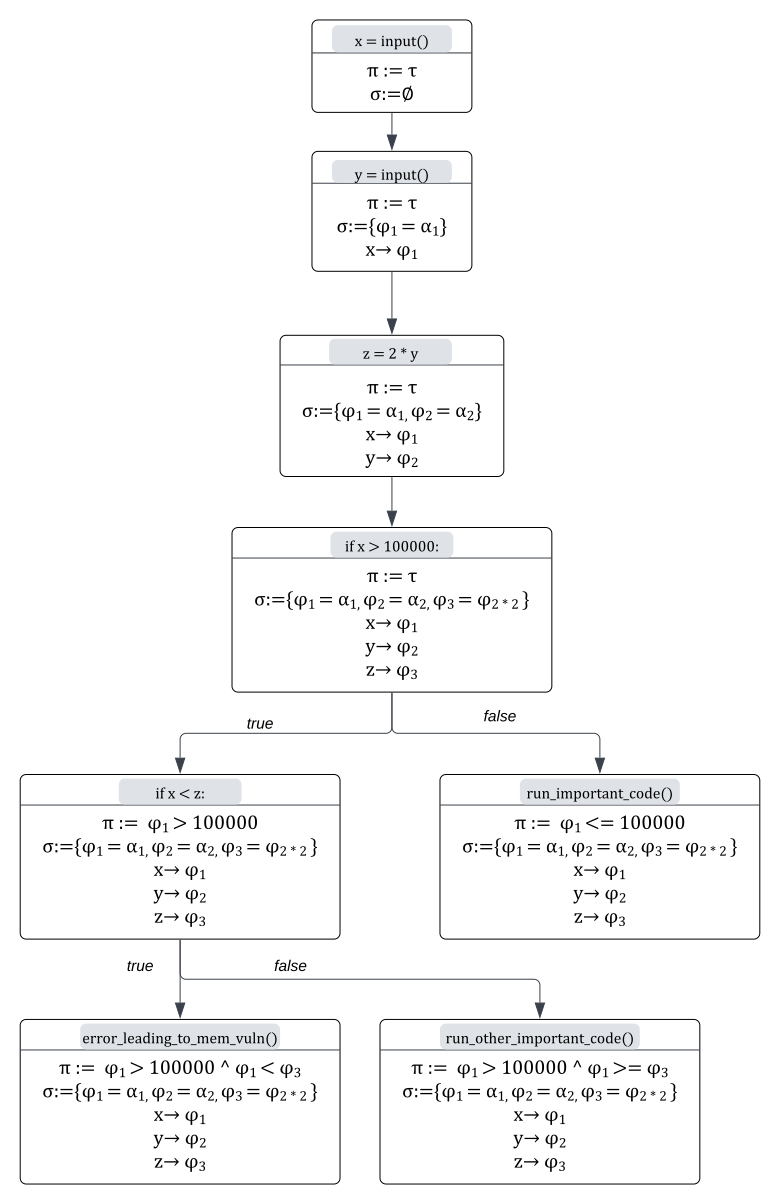
\includegraphics[scale=0.31]{figures/final_symbolic_example_graph.png}
        \caption{} % används för rendera b) som caption
        \label{fig:symbex_example_graph}
    \end{subfigure}

    \caption{Exempel för att visa symbolisk exekvering: pseudokod (a) och path
        constraint och symboliskt tillstånd för alla vägar i pseudokoden angett
        i (b). $  \mathcal{S} = \{\sigma := \{\phi_1 = \alpha_1, \phi_2 = \alpha_2, \phi_3 =
            2\phi_2\}, x \rightarrow \phi_1, y \rightarrow \phi_2, z \rightarrow
            \phi_3\}$}
\end{figure}

Exempelprogrammet i figur~\ref{fig:symbex_example_code} använder symbolisk
exekvering för att hitta vilken indata som leder programexekveringen till de
olika grenarna i programflödet. I många fall är det intressant att göra en
uttömmande sökning och hitta alla möjliga vägar i ett program, något som är
möjligt i detta program men inte i alla. Ett motexempel är komplexa
program som på grund av vägexplosionsproblemet inte hittar alla möjliga vägar.
Variablerna \emph{x} och \emph{y} sätts till symboliska värden som sedan används
för att beräkna vägvillkoret och de symboliska uttryck som variablerna utvecklas
till för en vald gren. Därefter används dessa uttryck och vägvillkor 
tillsammans för att bilda en ekvation som sedan kan lösas med hjälp av en SMT-lösare.
Figur~\ref{fig:symbex_example_graph} visar
hur det symboliska tillståndet förändras för alla möjliga grenar i programmet.

I~\ref{fig:symbex_example_graph} används $\pi$ för att ange vägvillkoret vilket
är initialt satt till $\top$ eftersom villkoret är sant från början och $\sigma$
används för att visa mappningen för symboliska värden. $\pi$ och $\sigma$ % något man kan använda ist för mappning kanske
populeras längs med exekveringen, och \emph{x} och \emph{y} mappas till
symboliska värden. Beroende på vilken väg som väljs i exekveringen, uppdateras
vägvillkoret. I andra noden sett uppifrån finns det två skillnader i jämförelse
med den första noden: \emph{x} tilldelas $\phi_1$ som är en symbolisk mappning
till $\alpha_1$. Efter den fjärde noden sett uppifrån görs ett val och
vägvillkoret förändras beroende på vilken väg som tas -- vägvillkoret uppdateras
till $\phi_1 > 100000$ om $x < z$ och annars uppdateras det till $\phi_1 \leq 
    100000$. På samma sätt uppdateras $\pi$ och $\phi$ längs andra exekveringsvägar
och vilket till slut leder till ett komplett programflödesdiagram som beror på
\emph{x, y, z}. I varje nod kan ett konkret värde som uppfyller vägvillkoren evalueras.

\section{Fuzzing}
Fuzzing är ett användbart automatiskt verktyg för att testa program efter
ofta svårupptäckta problem som minnesbuggar, krascher, etc. tack vare dess
enkelhet i att konfigurera verktyget mot godtyckliga program.  

Grundprincipen i fuzzing är att attackera en större mängd av möjlig indata genom
att generera oväntad, godtycklig eller felaktig data. Denna typ av genererad
indata resulterar ofta i syntaktiskt eller semantiskt felaktig indata som inte
kan hanteras av målprogrammet. Således finns det anledning för
utvecklingspotential, något som lett till bland annat mutation-based fuzzing och
generaton-based fuzzing. Mutation-based fuzzing muterar känd giltig indata,
t.ex. om strängen "fuzz" är giltig indata kan detta muteras till "fuzzZZZZZ". Om
en användare exempelvis vill fuzztesta bildhanteringsbiblioteket libjpeg skulle
detta innebära att skicka giltiga jpeg-bilder till fuzzern för att användas som
seeds, ett värde som används i en pseudoslumptalsgenerator för att generera ett
pseudoslumptal, och sedan modifiera dessa. Detta skiljer sig från
Generation-based fuzzing som genererar indata givet en modell för domänen -- en
fördel i jämförelse med mutation-based fuzzing som kräver känd kvalitativ
indata~\cite{fuzzing}. 

\subsection{Problem med fuzzing}
Ett problem är insikt om den underliggande kodstrukturen. En
viktig egenskap hos fuzzers som används för att beskriva dess effektivitet är
code coverage -- fuzzerns förmåga att traversera över samtliga kanter och noder i programmets
kontrollflödesgraf. Black-box fuzzing är ett exempel på en fuzzer
som saknar vetskap om den underliggande kodstrukturen och genererar
endast slumpmässig indata, något som leder till ytlig testning av målprogrammet.
I kontrast till black-box fuzzing finns det andra fuzzers, till exempel gray-box
fuzzern AFL~\cite{aflplusplus} som tillämpar binärinstrumentering, en teknik för att observera
eller manipulera en binär vilket görs genom att modifiera källkoden i binären.
Genom binärinstrumentering fås information om underliggande basic blocks som
delger övergången till nästa basic block. Detta används sedan av AFL för att ge
feedback till fuzzern som minns code coverage för en viss indata och repeterar
denna process för att maximera code coverage med ny indata och därmed öka
testytan~\cite{challenges_fuzzing}.

Fuzzers kräver ofta protokoll- eller domänkännedom för att kunna generera
indata. Detta blir problem för komplexa kodbaser eller bibliotek som saknar
trivial eller uppenbar indata och leder därmed till lägre code coverage.

\subsection{Symbolisk fuzzing}
Symbolisk fuzzing, eller concolic testing, är en white-box fuzzer som nyttjar
symbolisk exekvering för att nå maximal code coverage. Skiljt från gray-box
fuzzers som AFL, möjliggör symbolisk exekvering att fuzzern alltid väljer en
branch som inte tidigare tagits och således ökar code
coverage~\cite{challenges_fuzzing}.  


% vad är viktigt att veta om symbolisk fuzzing? hur används symbolisk
% exekvering? 
% hur används symbolisk exekvering?



\section{Exekveringsmotor}

Kärnan i ett korrekt dynamisk binäranalysverktyg är en \emph{exekveringsmotor},
en komponent som på ett korrekt vis kan exekvera programmet.
Figur~\ref{schematic} visar förhållandet mellan användaren, analysverktyget och
dess exekveringsmotor. Att köra ett program innebär att ladda binären och dess
bibliotek, hoppa till startadressen och sedan köra enskilda instruktioner. Om
binäranalysverktyget ska kunna använda metoder som använder symbolisk
exekvering behöver denna exekvering av enskilda instruktioner också stödja
symboliska variabler.


\begin{figure}[H]
    \centering
    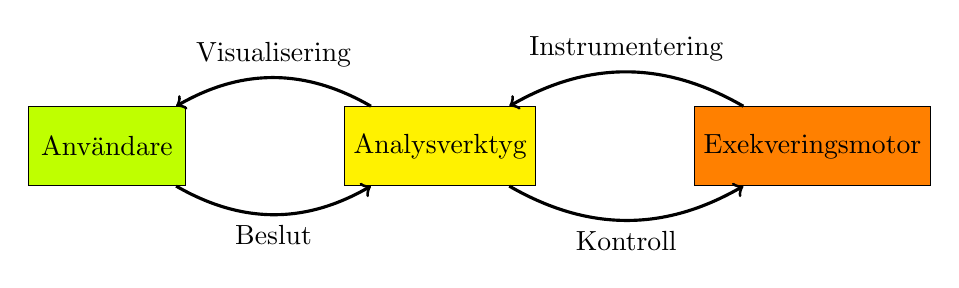
\begin{tikzpicture}

        \node [draw, fill=lime, minimum
            width=2cm, minimum height=1cm, ]  (user) {Användare};

        \node [draw, fill=yellow, minimum width=2cm, minimum height=1cm,
            right=2cm of user ] (tool) {Analysverktyg};

        \node [draw, fill=orange, minimum width=2cm, minimum height=1cm,
            right=2cm of tool ] (engine) {Exekveringsmotor};

        \draw[->, line width=.4mm] (user.-30) to[out=-30, in=-150]
        node[midway,below]{Beslut} (tool.-150);

        \draw[->, line width=.4mm] (tool.150) to[out=150, in=30]
        node[midway,above]{Visualisering} (user.30);

        \draw[->, line width=.4mm] (tool.-30) to[out=-30, in=-150]
        node[midway,below]{Kontroll} (engine.-150);

        \draw[->, line width=.4mm] (engine.150) to[out=150, in=30]
        node[midway,above]{Instrumentering} (tool.30);

    \end{tikzpicture}
    \caption{ Schematisk bild av ett binäranalysverktyg byggt kring en exekveringsmotor}\label{schematic}
\end{figure}

Symbolisk exekvering innehar, i praktiken, begränsningar i skalbarhet. En
symbolisk exekveringsmotor som utför symbolisk exekvering behöver ta hänsyn
till ett antal frågor gällande~\cite{survey_symb_exc}:

\paragraph{Minne} Motorn behöver spara komplexa datatyper och representera de
på ett sätt som tillåter villkorslösning. Exekvering av större program kräver
mer minne för att bokföra symboler och uttryck och därmed mer tid för
exekvering~\cite{survey_symb_exc}.

\paragraph{Miljö} Program i verkligheten kommunicerar på många sätt med sin
omgivning. För program är detta en virtuell miljö bestående av filer,
biblioteksanrop och IPC (\emph{inter process communication}). För att en
\textit{exekveringsmotor} ska vara så brett tillämpbar som möjligt behöver den
också stödja flera sorters omgivningskommunikation och representera omgivningen
på ett så komplett sätt som möjligt~\cite{survey_symb_exc}.

\paragraph{Stigexplotion} Verkliga program innehåller loopar, rekursion,
undantag och kombinationer av dessa som kan orsaka ett exponentiellt ökande
antal exekveringsvägar i programflödet. Det är alltså osannolikt att en motor
kan uttömmande utforska alla möjliga exekveringsvägar inom rimlig tid.
\emph{State-merging} kan appliceras i vissa fall för att begränsa antal
exekveringsvägar. \emph{State-merging} går ut på att slå samman ett antal
exekveringsvägar genom att upptäcka exekveringsvägar som liknar varandra och
slå samman dessa genom att kombinera dess villkor. Det krävs heuristik för att
upptäcka fall där \emph{state-merging} är applicerbart~\cite{survey_symb_exc}.

\paragraph{Villkorslösning} SMT-lösare kan skala till komplexa kombinationer av
villkor över hundratals variabler. Däremot kan icke-linjär aritmetik utgöra ett
stort hinder för effektivitet. Dessutom finns det exempel på olösliga problem
där SMT-lösare är inte tillämpbara~\cite{survey_symb_exc}.

% \subsection{Analyser}
%
% Det finns många möjliga analyser som kan användas av ett binäranalysverktyg, där
% \textit{analyser} avser en visualisering av en aspekt av det analyserade
% programmets beteende eventuellt inklusive ett sätt för användaren att påverka
% det analyserade programmets körning.
%
% En konkret exekvering kan spåras och dess instruktionssekvens kan visas för
% användaren med loopar identifierade. Flera exekveringar kan visualiseras på
% samma sätt och deras instruktionssekvenser användas för att återskapa
% kontrollflödesstrukturer som for- och while-loopar och if-satser.
%
% Möjligheter för \textit{state merging} kan identifieras helautomatiskt eller av
% användaren, alltså platser där flera exekveringar kan ersättas av en enda mer
% generell exekvering som innehåller ursprungsexekveringarnas skillnader som
% symboliska uttryck.
%
% En uppsättning liknande exekveringar kan visas upp för användaren tillsammans
% med information om när och hur de divergerar, för att till exempel avgöra när
% olika delar av indatan används.
%
% För analys av programmet är det också hjälpsamt för användaren att kunna stega
% genom exekveringen steg för steg och ändra på värden för att ta de vägar de vill
% analysera. Detta borde också kunna göras baklänges, det vill säga att användaren
% väljer en slutdestination och låter programmet själv lista ut vilka värden som
% behövdes läsas för att exekveringen skulle ta sig till den punkten.
%
% En mer automatisk men ändå viktig funktionalitet är konstruktion av kod-täckande
% indata. När testfall som besöker en uppsättning instruktioner är konstruerad kan
% kraven på indatan över denna uppsättning programhopp analyseras och programmet
% kan lista ut vilka aspekter av indatan som kan ändras utan att påverka
% kodtäckningsgraden, och kommunicera detta till användaren.
%
% Det finns många möjliga analyser. Användbarheten i ett verktyg mäts inte i
% kvantiteten analyser utan i förmågan för de utvalda implementerade analyserna
% att täcka användarens behov av förståelse av programmet.


\chapter{Existerande verktyg}\label{chap:existerande_verktyg}
För att evaluera verktyget används existerande verktyg som jämförelse i
kombination med att dess fördelar och nackdelar vägs mot AMBA. Dessutom
presenteras en diskussion kring utvecklingsprocessens gång och
vidareutvecklingspotential.

\section{Jämförelse mellan AMBA och Ghidra} Ghidra är ett avancerat verktyg som
gör statisk analys bortom syftet med AMBA, men AMBA har ett par likheter. Ghidra
kan representera en kontrollflödesgraf för en given binär på två olika sätt:
\textit{Flow Graph} och \textit{Code Flow Graph}~\cite{ghidra_website}.

\begin{figure}[H]
    \begin{subfigure}{0.3\textwidth}
        \includegraphics[width=\linewidth]{figures/ghidra_code_listing.png}
        \caption{Ghidras code listing.} \label{fig:ghidra_code_listing}
    \end{subfigure}
    \hspace*{\fill}
    \begin{subfigure}{0.3\textwidth}
        \includegraphics[width=\linewidth]{figures/ghidra_block_flow_graph.png}
        \caption{Ghidras block-flow-graph.}
        \label{fig:ghidra_block_graph}
    \end{subfigure}
    \hspace*{\fill}
    \begin{subfigure}{0.3\textwidth}
        \includegraphics[width=\linewidth]{figures/ghidra_code_flow.png}
        \caption{Ghidras code-flow-graph.} \label{fig:ghidra_code_flow_graph}
    \end{subfigure}

    \caption{Tre primära vyer i verktyget Ghidra för att representera ett programs
        kontrollflödesgraf.} \label{fig:ghidra_figures}
\end{figure}

Ghidra kompletterar dessa vyer med en \textit{code listing}, en primär vy där
binärens disassemblerade kod listas. Användaren kan fritt välja att bilda en
graf från ett markerat \textit{code block}, vilket är Ghidras utökade
specifikation på ett basic block, från Ghidras code
listing~\cite{ghidra_website}. AMBA har liknande funktionalitet, se
figur~\ref{fig:graf-basic}, och kan visualisera binärens fullständiga
disassemblerade kod för en given nod, om debugdata finns tillgänglig, men saknar
större kontext likt Ghidras code listing. En fördel mot Ghidras representation
är AMBAs tre olika sätt att representera en binärs kontrollflöde på: \textit{Raw
    Basic Block Graph}, \textit{Compressed Block Graph}, och \textit{State Graph}.
Genom att använda dessa tre olika vyer kan en användare bilda en större
förståelse om en given binär, dels genom att exempelvis visualisera alla
symboliska tillstånd som \stoe{} skapar i kombination med färgade noder som
indikerar på starkt kopplade komponenter (jfr. eng. \emph{strongly connected
    components}).

Kännedom om starkt kopplade komponenter i en kontrollflödesgraf är i synnerhet
intressant vid analys av binärer utan källkod, eftersom dessa delgrafer speglar
en starkare koppling mellan noderna och indikerar på en sektion i binären som
troligtvis har större relevans än en sektion som saknar eller har betydligt
färre starkt kopplade komponenter. Ett typiskt mönster man kan se med starkt
kopplade komponenter är icke-nestlade loopar.

En användare skulle exempelvis kunna använda AMBAs node colouring för att bilda
en större uppfattning om en viss del i binären och sedan komplettera med
nodernas minnesaddresser för att visualisera samma sektion i ett mer avancerat
verktyg som Ghidra. Ett typiskt användningsfall skulle kunna vara att i Ghidra
söka efter strängar som ger mer information i den givna kodsektionen från AMBA
eller använda Ghidras analysmetoder för att dekompilera binärens instruktioner
till ett mer läsbart format i form av pseudokod.

\section{Jämförelse mellan S2E och Angr som \\ backend} Eftersom AMBA använder
\stoe{} som symbolisk exekveringsmotor har AMBA således en teoretisk fördel i
prestanda, något som kan avläsas från figurerna
i~\cite[Figur~1-5]{systematic_comparison_symbex}. Delvis beror detta på att Angr
är skrivet i python som är ett interpreterat språk och \stoe{} som är skrivet i
C++ som är ett kompilerat språk. Detta innebär att AMBA inte nödvändigtvis i
nuläget har bättre prestanda mot applikationer utvecklade med Angr som
\emph{backend}. Dock betyder det att AMBA har en teoretisk konkurrenskraftig
prestanda.

Angr är dock ett mer flexibelt verktyg som har den funktionalitet som \stoe{}
tillhandahåller, och är dessutom i allmänhet enklare att påbörja utveckling med
och onekligen eklare att bygga. Dessutom är Angr i synnerhet ett eftertraktat
verktyg att använda som symbolisk exekveringsmotor eftersom det bland annat
tillhandahåller funktionalitet såsom \emph{Control-Flow Graph Recovery} och
disassemblering som möjliggör mycket av funktionalitet som annars behövdes
implementeras i AMBA.

\section{Jämförelse mellan AMBA och SymNav} SymNav tillhandahåller samma
funktionalitet som AMBA gör bortsett från en detalj: användare kan genom SymNav
ta bort states som inte är intressanta medan i AMBA kan användare prioritera
states som ska analyseras. Dessutom presenteras funktionaliteten i SymNav på ett
mer användarvänligt sätt: vyn splittar upp respektive funktionalitet i
applikationen och presenterar detta i stil med designmönstret \emph{Grid of
    equals}.

Utöver detta är den stora skillnaden vilken symbolisk exekveringsmotor som
används. SymNav använder Angr, och AMBA använder, som tidigare nämnt, \stoe{}
vilket innebär att SymNav får en enklare kodbas eftersom mycket av koden som
interagerar med Angr är pythonskript likt API-anrop vilket kräver mindre total
kod för att uppnå samma sak som med \stoe{} men är istället begränsad i
skalbarhet. \stoe{} har inbyggda plugins som tillhandahåller mycket
funktionalitet, till exempel \emph{ExecutionTracer} som övervakar och
registrerar information längs med exekveringen för en given branch vilket
tillåter en att undersöka vad som orsakar path explosion eller vilken branch som
gör flest förgreningar.

\section{Arbetsprocess}
Eftersom \stoe{} är ett komplext system med många komplicerade
biblioteksberoenden ansågs det tidigt i arbetsprocessen att göra AMBA mer
tillgängligt till slutanvändaren genom att paketera alla bibliotek som krävs för
att köra \stoe{}. Detta var en komplicerad och tidskrävande uppgift eftersom
mycket av \stoe{}s byggsystem var tvunget att återimplementeras eller kringgås
när tvetydiga och icke-triviala problem uppstod. Ett sådant problem var
nedladdningen och byggningen av guest images som \stoe{} lagrades på google
drive där lösningen var att istället ladda ner färdiga guest images.

Denna del av arbetet ledde till att mycket av planeringen blev förskjutet och
således fanns det mindre tid till att utveckla all funktionalitet som var tänkt.

\section{Vidareutveckling}
En särskilt eftertraktad funktionalitet är \textit{State merging}. Syftet med
state merging är att minska antalet exekveringsvägar genom att förena symboliska
tillstånd som är ekvivalenta. Genom att introducera state merging ökar
prestandan för den symboliska exekveringen som gör det möjligt att skicka fler
förfrågningar (jfr. eng. \emph{queries}) till SMT-lösaren.

Övervakning av systemanrop (jfr. eng. \emph{syscalls}) ger användaren en större
insikt i vad som sker i en specifik del av grafen, exempelvis om det sker
inmatning eller utmatning, om en process signaleras att stängas av, om binären
kör ett exec-systemanrop för att köra ett externt program, etc. är anledningar
som gör det intressant att övervaka systemanrop. För att implementera detta i
AMBA bör det undersökas om det finns hooks för detta.

I nuläget sparas inte resultatet från SMT-lösaren för ett givet path constraint
och därför får användaren inte heller mer informatiom om vilken input som ledde
till att vägen nåddes i exekveringen. Optimalt hade varit om användaren kunde se
vilken indata som ledde till en särskild väg för fortsatt analys. \stoe{} har
denna information, men i nuläget sparas den inte av AMBA.


\section{Statisk disassemblering}\label{sec:existerande-disasm}
Ghidra är ett \emph{reverse engingeering} ramverk utvecklat av USA:s NSA
(National Security Agency) och kan disassembla en binär till pseudo-C-kod.
Ghidra har också en debugger och funktionsgraf. Debuggern ska underlätta binär
debugging genom att integrera med andra funktioner i Ghidra. Funktionsgrafen
låter användaren se hur programmet är uppbyggt visuellt och hur olika
funktioner interagerar med varandra. Funktionaliteter kan utökas eller andra
funktioner utvecklas genom plugins till Ghidra\cite{ghidra_use_cases}. Ghidra
tillåter även automatisering genom att skriva skript. Ett exempel är ett skript
som hittar exempelvis sårbarhet i form av funktionsanrop till potentiellt
osäkra API-anrop genom statisk analys\cite{ghidra_script}.

\section{Dynamiska binäranalysramverk för symbolisk exekvering}\label{sec:existerande-ramverk}
En metod för dynamisk binäranalys är symbolisk exekvering. Eftersom exekveringen är symbolisk är
det möjligt att utforska alla möjliga exekveringsvägar i programmet, även de som inte är möjliga
med konkreta inputs. Både \stoe{} och SymQEMU är kraftfulla verktyg för att analysera binära program
med symbolisk exekvering.

SymQEMU är byggt som en förlängning av QEMU, och använder en kombination av dynamisk binär
översättning och symbolisk exekvering för att analysera binära program som körs inuti emulatorn.
SymQEMU utför kompileringsbaserad symbolisk exekvering, där den mellanliggande representationen först blir modifierad
innan den översätts till värdarkitekturen, och är därför arkitekturoberoende utan att påverka prestandan~\cite{symqemu}.

\stoe{} är ett modulärt bibliotek som ger virtuella maskiner symbolisk exekvering. \stoe{} erbjuder
redskap för att fokusera utforskningen på delkomponenter av systemet och gör det även
möjligt för användare att sätta in kod i målsystemet vid specifika punkter under
exekvering. Det gör att användare kan anpassa analysprocessen efter sina behov~\cite{s2e}.
\stoe{} kan analysera kod för de flesta processorarkitekturer men betalar för det med ökad
komplexitet och prestanda~\cite{symqemu}.

Ett annat verktyg för att identifiera buggar och sårbarheter med hjälp av dynamisk symbolisk
exekvering är SAGE (Scalable Automated Guided Execution).
SAGE var det första verktyget som utförde dynamisk symbolisk exekvering på x86-binärnivå och använder flera
avgörande optimeringar för att hantera stora exekverings-spår (jmf.\ engelska execution traces).
För att skala upp till stora exekverings-spår använder SAGE flera tekniker för att förbättra hastigheten och
minnesanvändningen för constraint generering, exempelvis så kartläggs ekvivalenta symboliska uttryck till samma
objekt och constraints som redan är tillagda hoppas över~\cite{sage}.

Ett binäranalysverktyg med stöd för både statiska och dynamiska analyser
med hjälp av symbolisk exekvering är angr. Verktyget är ett ramverk för binäranalys och 
har stöd för disassemblering till pseudo-C-kod och många analyser man kan utföra.
Baserat på en emulator skriven i Python, stödjer angr symbolisk exekvering och 
analyser utförs genom Python-skript som interagerar med angrs API."\@ angr har
använts för att framställa skript som kan utföra \emph{reverse engineering},
sårbarhetssökning och fungera som exploateringsverktyg~\cite{angr_docs}. År 2016 
så vann ett system som heter Mayhem, som använde angr som symbolisk 
exekveringsmotor, Cyber Grand Challenge, som hålls av the Defense Advanced Research 
Projects Agency (DARPA). 

För att accelerera den symboliska exekveringen kan angr användas i kombination 
med Unicorn CPU-emulatorn, ett lättviktigt ramverk för emulering som stödjer 
många arkitekturer och baseras på QEMU~\cite{UnicornEngine}. Detta är möjligt 
med hjälp av komponenten \emph{angr.engines.unicorn}. Genom att använda komponenten 
kan man exekvera med konkreta input när det är möjligt och fördelaktigt men stödja 
detta med symbolisk exekvering då flera exekveringsvägar behöver utforskas 
eller programmets beteende inte är deterministiskt~\cite{angr_uni}. 


\section{Automatiska fuzzers}\label{sec:existerande-automatisk}
Ytterligare en metod för binäranalys är fuzzing. Fuzzing innebär att testa ett
program med en stor mängd olika input. Målet är att simulera oväntade beteenden
eller krashar om potentialen för dessa existerar. Fuzzing är därför ett
effektivt medel för att undersöka om ett program innehåller
sårbarheter~\cite{rawat}.

AFL++ är en utveckling av den ursprungliga AFL (American Fuzzy Lop) fuzzern och
har förbättrats med fler funktioner och bättre prestanda. AFL använder
täckningsstyrd fuzzing (jmf.\ engelska coverage-guided fuzzing) för att generera
testfall som är troliga att utlösa buggar och sårbarheter. AFL spårar
kodtäckningen vid varje testfall och använder denna informationen för att styra
hur tidigare testfall mutateras till nya. Även AFL++ muterar input för att
generera nya inputs från befintliga, och använder feedback från programvaran som
fuzzas för att styra fuzzing-processen~\cite{aflplusplus}.

\section{Visualiserad symbolisk fuzzing}\label{sec:existerande-visualiserad}
De i avsnitt~\ref{sec:befintliga-disasm},\ \ref{sec:befintliga-ramverk} samt\
\ref{sec:befintliga-automatisk} presenterade kategorierna av binäranalysverktyg
är alla etablerade kategorier som AMBA inte faller under. Kategorin som AMBA
tillhör kallar vi ''visualiserad symbolisk fuzzing'' och detta avsnitt
diskuterar det fåtal befintliga verktyg som vi anser faller inom kategorin.

Verktyget Symbolic Execution Debugger
(SED)~\cite{symbolic_execution_debugger} är en debugger för Java 1.4
utan multitrådning, reflektion och flyttalsaritmetik. Användaren använder
SED som ett Eclipse-plugin, i vilket valfri metod kan väljas och
analyseras med symbolisk exekvering. Exekveringsträdet visas för användaren
tillsammans med källkodsrader och de vägvillkor som tar exekveringen dit.

Att SED är utformat som en debugger som kan starta exekveringen vid
valfri Javametod gör verktyget väl utformat till formell verifiering. Verktyget
förlitar sig på tillgång till källkod och att användaren vet vilken indata som
anses giltig för metoden. Begränsningen till enskilda metoder gör samtidigt den
symboliska exekveringen mer överblicklig för användaren, då användaren i mindre
grad själv behöver exkludera det som analysen inte bör lägga fokus på.

Att SED inriktar sig på en delmängd av Java innebär att det är mindre
applicerbart för datasäkerhet och binäranalys då dessa sammanhang ofta kräver
analys av exekverbara binärer, ofta utan tillgång till källkod. Eftersom Java är
ett språk på högre nivå än maskinkod innebär samtidigt en inriktning mot Java
att många implementationsdetaljer i hur koden skulle göras på en riktig dator
kan ignoreras. Dynamisk minneshantering är ett exempel på detta, där analys av
Javakod kan abstrahera bort exekveringsmiljöns anrop till \verb|malloc()| och
\verb|free()| medan analys av maskinkod nödvändigtvis behöver hantera
komplexiteten i deras implementationer. Symbolisk exekvering i en högnivåmiljö
exkluderar därmed också många detaljer som verktyget eller användaren annars på
annat vis hade behövt filtrera bort.

Verktyget SymNav~\cite{symnav} kan visualisera och kontrollera analysen av en
exekverbar binär inuti angr:s symboliska exekveringsmotor.\@ angr beskrivs i
avsnitt~\ref{sec:befintliga-ramverk}.

Arbetsflödet består av att starta SymNav med en via kommandorad angiven binär
och sedan vänta tills programmet forkar. Då visar det grafiska gränssnittet det
symboliska trädet, delar av kontrollflödesgrafen, etc. Användaren kan då
navigera den visualiserade informationen, och sedan antingen fortsätta eller
starta om körningen med en angiven tidsbudget och minnesbudget. Till exempel kan
användaren starta en sökning med standardparametrar i $10$ sekunder och med
$\SI{1}{\giga\byte}$ RAM.\@ När söktiden löpt ut uppdateras informationen i
det grafiska gränssnittet.

SymNavs grafiska gränssnitt består av tre paneler: en trädpanel som visar trädet
av symboliska tillstånd, en kontrollflödespanel som visar kontrollflödesgrafen
för enskilda funktioner och en styrpanel för att filtrera vilken information som
ska visas.

Trädpanelen visar en kompakt representation av alla vägar av symboliska
tillstånd som tagits. Dessutom visas en parallellkoordinatgraf där diverse
nyckeltal för de symboliska tillstånden visas. Genom att interagera med denna
graf kan användaren filtrera bort vägar efter nyckeltal, till exempel genom att
endast visa vägar som någon gång anropar \verb|malloc()|.

Kontrollflödespanelen visar en graf över alla grundblock inom en funktion. Noder
innehåller den assemblykod som deras grundblock innehåller och kanter färgläggs
efter hur många olika symboliska tillstånd som vandrat kanten.

Styrpanelen visar för användaren vilka filter de hittills applicerat och låter
användaren filtrera ytterligare vilka symboliska tillstånd som ska visas i det
grafiska gränssnittet. Dessutom låter styrpanelen användaren definera
resursbudgeten, starta om körningen eller fortsätta körningen från nuvarande
symboliska tillstånd. När en körning startas kan användaren ange att nuvarande
filter i det grafiska gränssnittet ska omvandlas till villkor på den symboliska
indatan samt prioriteringsregler för fortsatt sökning.

SymNav är därmed fasbaserad, med alternerande söknings- och presentationsfaser.
SymNav ger användaren kraftfulla verktyg att filtrera ut intressanta tillstånd
efter metriker såsom kodtäckningsgrad och minnesallokeringsmönster. Samtidigt
ärver SymNav flera nackdelar från angr, såsom suboptimal prestanda
\cite{systematic_comparison_symbex} och begränsad miljömodellering då
analysgränsen går vid processen med emulerade systemanrop snarare än vid en
virtuell maskin. SymNav är skrivet för att kunna anpassas till andra
exekveringsmotorer än angr, men detta är inte implementerat i dess nuvarande
form.


\chapter{AMBA}\label{chap:amba}
För att evaluera verktyget används existerande verktyg som jämförelse i
kombination med att dess fördelar och nackdelar vägs mot AMBA. Dessutom
presenteras en diskussion kring utvecklingsprocessens gång och
vidareutvecklingspotential.

\section{Jämförelse mellan AMBA och Ghidra} Ghidra är ett avancerat verktyg som
gör statisk analys bortom syftet med AMBA, men AMBA har ett par likheter. Ghidra
kan representera en kontrollflödesgraf för en given binär på två olika sätt:
\textit{Flow Graph} och \textit{Code Flow Graph}~\cite{ghidra_website}.

\begin{figure}[H]
    \begin{subfigure}{0.3\textwidth}
        \includegraphics[width=\linewidth]{figures/ghidra_code_listing.png}
        \caption{Ghidras code listing.} \label{fig:ghidra_code_listing}
    \end{subfigure}
    \hspace*{\fill}
    \begin{subfigure}{0.3\textwidth}
        \includegraphics[width=\linewidth]{figures/ghidra_block_flow_graph.png}
        \caption{Ghidras block-flow-graph.}
        \label{fig:ghidra_block_graph}
    \end{subfigure}
    \hspace*{\fill}
    \begin{subfigure}{0.3\textwidth}
        \includegraphics[width=\linewidth]{figures/ghidra_code_flow.png}
        \caption{Ghidras code-flow-graph.} \label{fig:ghidra_code_flow_graph}
    \end{subfigure}

    \caption{Tre primära vyer i verktyget Ghidra för att representera ett programs
        kontrollflödesgraf.} \label{fig:ghidra_figures}
\end{figure}

Ghidra kompletterar dessa vyer med en \textit{code listing}, en primär vy där
binärens disassemblerade kod listas. Användaren kan fritt välja att bilda en
graf från ett markerat \textit{code block}, vilket är Ghidras utökade
specifikation på ett basic block, från Ghidras code
listing~\cite{ghidra_website}. AMBA har liknande funktionalitet, se
figur~\ref{fig:graf-basic}, och kan visualisera binärens fullständiga
disassemblerade kod för en given nod, om debugdata finns tillgänglig, men saknar
större kontext likt Ghidras code listing. En fördel mot Ghidras representation
är AMBAs tre olika sätt att representera en binärs kontrollflöde på: \textit{Raw
    Basic Block Graph}, \textit{Compressed Block Graph}, och \textit{State Graph}.
Genom att använda dessa tre olika vyer kan en användare bilda en större
förståelse om en given binär, dels genom att exempelvis visualisera alla
symboliska tillstånd som \stoe{} skapar i kombination med färgade noder som
indikerar på starkt kopplade komponenter (jfr. eng. \emph{strongly connected
    components}).

Kännedom om starkt kopplade komponenter i en kontrollflödesgraf är i synnerhet
intressant vid analys av binärer utan källkod, eftersom dessa delgrafer speglar
en starkare koppling mellan noderna och indikerar på en sektion i binären som
troligtvis har större relevans än en sektion som saknar eller har betydligt
färre starkt kopplade komponenter. Ett typiskt mönster man kan se med starkt
kopplade komponenter är icke-nestlade loopar.

En användare skulle exempelvis kunna använda AMBAs node colouring för att bilda
en större uppfattning om en viss del i binären och sedan komplettera med
nodernas minnesaddresser för att visualisera samma sektion i ett mer avancerat
verktyg som Ghidra. Ett typiskt användningsfall skulle kunna vara att i Ghidra
söka efter strängar som ger mer information i den givna kodsektionen från AMBA
eller använda Ghidras analysmetoder för att dekompilera binärens instruktioner
till ett mer läsbart format i form av pseudokod.

\section{Jämförelse mellan S2E och Angr som \\ backend} Eftersom AMBA använder
\stoe{} som symbolisk exekveringsmotor har AMBA således en teoretisk fördel i
prestanda, något som kan avläsas från figurerna
i~\cite[Figur~1-5]{systematic_comparison_symbex}. Delvis beror detta på att Angr
är skrivet i python som är ett interpreterat språk och \stoe{} som är skrivet i
C++ som är ett kompilerat språk. Detta innebär att AMBA inte nödvändigtvis i
nuläget har bättre prestanda mot applikationer utvecklade med Angr som
\emph{backend}. Dock betyder det att AMBA har en teoretisk konkurrenskraftig
prestanda.

Angr är dock ett mer flexibelt verktyg som har den funktionalitet som \stoe{}
tillhandahåller, och är dessutom i allmänhet enklare att påbörja utveckling med
och onekligen eklare att bygga. Dessutom är Angr i synnerhet ett eftertraktat
verktyg att använda som symbolisk exekveringsmotor eftersom det bland annat
tillhandahåller funktionalitet såsom \emph{Control-Flow Graph Recovery} och
disassemblering som möjliggör mycket av funktionalitet som annars behövdes
implementeras i AMBA.

\section{Jämförelse mellan AMBA och SymNav} SymNav tillhandahåller samma
funktionalitet som AMBA gör bortsett från en detalj: användare kan genom SymNav
ta bort states som inte är intressanta medan i AMBA kan användare prioritera
states som ska analyseras. Dessutom presenteras funktionaliteten i SymNav på ett
mer användarvänligt sätt: vyn splittar upp respektive funktionalitet i
applikationen och presenterar detta i stil med designmönstret \emph{Grid of
    equals}.

Utöver detta är den stora skillnaden vilken symbolisk exekveringsmotor som
används. SymNav använder Angr, och AMBA använder, som tidigare nämnt, \stoe{}
vilket innebär att SymNav får en enklare kodbas eftersom mycket av koden som
interagerar med Angr är pythonskript likt API-anrop vilket kräver mindre total
kod för att uppnå samma sak som med \stoe{} men är istället begränsad i
skalbarhet. \stoe{} har inbyggda plugins som tillhandahåller mycket
funktionalitet, till exempel \emph{ExecutionTracer} som övervakar och
registrerar information längs med exekveringen för en given branch vilket
tillåter en att undersöka vad som orsakar path explosion eller vilken branch som
gör flest förgreningar.

\section{Arbetsprocess}
Eftersom \stoe{} är ett komplext system med många komplicerade
biblioteksberoenden ansågs det tidigt i arbetsprocessen att göra AMBA mer
tillgängligt till slutanvändaren genom att paketera alla bibliotek som krävs för
att köra \stoe{}. Detta var en komplicerad och tidskrävande uppgift eftersom
mycket av \stoe{}s byggsystem var tvunget att återimplementeras eller kringgås
när tvetydiga och icke-triviala problem uppstod. Ett sådant problem var
nedladdningen och byggningen av guest images som \stoe{} lagrades på google
drive där lösningen var att istället ladda ner färdiga guest images.

Denna del av arbetet ledde till att mycket av planeringen blev förskjutet och
således fanns det mindre tid till att utveckla all funktionalitet som var tänkt.

\section{Vidareutveckling}
En särskilt eftertraktad funktionalitet är \textit{State merging}. Syftet med
state merging är att minska antalet exekveringsvägar genom att förena symboliska
tillstånd som är ekvivalenta. Genom att introducera state merging ökar
prestandan för den symboliska exekveringen som gör det möjligt att skicka fler
förfrågningar (jfr. eng. \emph{queries}) till SMT-lösaren.

Övervakning av systemanrop (jfr. eng. \emph{syscalls}) ger användaren en större
insikt i vad som sker i en specifik del av grafen, exempelvis om det sker
inmatning eller utmatning, om en process signaleras att stängas av, om binären
kör ett exec-systemanrop för att köra ett externt program, etc. är anledningar
som gör det intressant att övervaka systemanrop. För att implementera detta i
AMBA bör det undersökas om det finns hooks för detta.

I nuläget sparas inte resultatet från SMT-lösaren för ett givet path constraint
och därför får användaren inte heller mer informatiom om vilken input som ledde
till att vägen nåddes i exekveringen. Optimalt hade varit om användaren kunde se
vilken indata som ledde till en särskild väg för fortsatt analys. \stoe{} har
denna information, men i nuläget sparas den inte av AMBA.



\chapter{Implementation}\label{chap:implementation}
För att evaluera verktyget används existerande verktyg som jämförelse i
kombination med att dess fördelar och nackdelar vägs mot AMBA. Dessutom
presenteras en diskussion kring utvecklingsprocessens gång och
vidareutvecklingspotential.

\section{Jämförelse mellan AMBA och Ghidra} Ghidra är ett avancerat verktyg som
gör statisk analys bortom syftet med AMBA, men AMBA har ett par likheter. Ghidra
kan representera en kontrollflödesgraf för en given binär på två olika sätt:
\textit{Flow Graph} och \textit{Code Flow Graph}~\cite{ghidra_website}.

\begin{figure}[H]
    \begin{subfigure}{0.3\textwidth}
        \includegraphics[width=\linewidth]{figures/ghidra_code_listing.png}
        \caption{Ghidras code listing.} \label{fig:ghidra_code_listing}
    \end{subfigure}
    \hspace*{\fill}
    \begin{subfigure}{0.3\textwidth}
        \includegraphics[width=\linewidth]{figures/ghidra_block_flow_graph.png}
        \caption{Ghidras block-flow-graph.}
        \label{fig:ghidra_block_graph}
    \end{subfigure}
    \hspace*{\fill}
    \begin{subfigure}{0.3\textwidth}
        \includegraphics[width=\linewidth]{figures/ghidra_code_flow.png}
        \caption{Ghidras code-flow-graph.} \label{fig:ghidra_code_flow_graph}
    \end{subfigure}

    \caption{Tre primära vyer i verktyget Ghidra för att representera ett programs
        kontrollflödesgraf.} \label{fig:ghidra_figures}
\end{figure}

Ghidra kompletterar dessa vyer med en \textit{code listing}, en primär vy där
binärens disassemblerade kod listas. Användaren kan fritt välja att bilda en
graf från ett markerat \textit{code block}, vilket är Ghidras utökade
specifikation på ett basic block, från Ghidras code
listing~\cite{ghidra_website}. AMBA har liknande funktionalitet, se
figur~\ref{fig:graf-basic}, och kan visualisera binärens fullständiga
disassemblerade kod för en given nod, om debugdata finns tillgänglig, men saknar
större kontext likt Ghidras code listing. En fördel mot Ghidras representation
är AMBAs tre olika sätt att representera en binärs kontrollflöde på: \textit{Raw
    Basic Block Graph}, \textit{Compressed Block Graph}, och \textit{State Graph}.
Genom att använda dessa tre olika vyer kan en användare bilda en större
förståelse om en given binär, dels genom att exempelvis visualisera alla
symboliska tillstånd som \stoe{} skapar i kombination med färgade noder som
indikerar på starkt kopplade komponenter (jfr. eng. \emph{strongly connected
    components}).

Kännedom om starkt kopplade komponenter i en kontrollflödesgraf är i synnerhet
intressant vid analys av binärer utan källkod, eftersom dessa delgrafer speglar
en starkare koppling mellan noderna och indikerar på en sektion i binären som
troligtvis har större relevans än en sektion som saknar eller har betydligt
färre starkt kopplade komponenter. Ett typiskt mönster man kan se med starkt
kopplade komponenter är icke-nestlade loopar.

En användare skulle exempelvis kunna använda AMBAs node colouring för att bilda
en större uppfattning om en viss del i binären och sedan komplettera med
nodernas minnesaddresser för att visualisera samma sektion i ett mer avancerat
verktyg som Ghidra. Ett typiskt användningsfall skulle kunna vara att i Ghidra
söka efter strängar som ger mer information i den givna kodsektionen från AMBA
eller använda Ghidras analysmetoder för att dekompilera binärens instruktioner
till ett mer läsbart format i form av pseudokod.

\section{Jämförelse mellan S2E och Angr som \\ backend} Eftersom AMBA använder
\stoe{} som symbolisk exekveringsmotor har AMBA således en teoretisk fördel i
prestanda, något som kan avläsas från figurerna
i~\cite[Figur~1-5]{systematic_comparison_symbex}. Delvis beror detta på att Angr
är skrivet i python som är ett interpreterat språk och \stoe{} som är skrivet i
C++ som är ett kompilerat språk. Detta innebär att AMBA inte nödvändigtvis i
nuläget har bättre prestanda mot applikationer utvecklade med Angr som
\emph{backend}. Dock betyder det att AMBA har en teoretisk konkurrenskraftig
prestanda.

Angr är dock ett mer flexibelt verktyg som har den funktionalitet som \stoe{}
tillhandahåller, och är dessutom i allmänhet enklare att påbörja utveckling med
och onekligen eklare att bygga. Dessutom är Angr i synnerhet ett eftertraktat
verktyg att använda som symbolisk exekveringsmotor eftersom det bland annat
tillhandahåller funktionalitet såsom \emph{Control-Flow Graph Recovery} och
disassemblering som möjliggör mycket av funktionalitet som annars behövdes
implementeras i AMBA.

\section{Jämförelse mellan AMBA och SymNav} SymNav tillhandahåller samma
funktionalitet som AMBA gör bortsett från en detalj: användare kan genom SymNav
ta bort states som inte är intressanta medan i AMBA kan användare prioritera
states som ska analyseras. Dessutom presenteras funktionaliteten i SymNav på ett
mer användarvänligt sätt: vyn splittar upp respektive funktionalitet i
applikationen och presenterar detta i stil med designmönstret \emph{Grid of
    equals}.

Utöver detta är den stora skillnaden vilken symbolisk exekveringsmotor som
används. SymNav använder Angr, och AMBA använder, som tidigare nämnt, \stoe{}
vilket innebär att SymNav får en enklare kodbas eftersom mycket av koden som
interagerar med Angr är pythonskript likt API-anrop vilket kräver mindre total
kod för att uppnå samma sak som med \stoe{} men är istället begränsad i
skalbarhet. \stoe{} har inbyggda plugins som tillhandahåller mycket
funktionalitet, till exempel \emph{ExecutionTracer} som övervakar och
registrerar information längs med exekveringen för en given branch vilket
tillåter en att undersöka vad som orsakar path explosion eller vilken branch som
gör flest förgreningar.

\section{Arbetsprocess}
Eftersom \stoe{} är ett komplext system med många komplicerade
biblioteksberoenden ansågs det tidigt i arbetsprocessen att göra AMBA mer
tillgängligt till slutanvändaren genom att paketera alla bibliotek som krävs för
att köra \stoe{}. Detta var en komplicerad och tidskrävande uppgift eftersom
mycket av \stoe{}s byggsystem var tvunget att återimplementeras eller kringgås
när tvetydiga och icke-triviala problem uppstod. Ett sådant problem var
nedladdningen och byggningen av guest images som \stoe{} lagrades på google
drive där lösningen var att istället ladda ner färdiga guest images.

Denna del av arbetet ledde till att mycket av planeringen blev förskjutet och
således fanns det mindre tid till att utveckla all funktionalitet som var tänkt.

\section{Vidareutveckling}
En särskilt eftertraktad funktionalitet är \textit{State merging}. Syftet med
state merging är att minska antalet exekveringsvägar genom att förena symboliska
tillstånd som är ekvivalenta. Genom att introducera state merging ökar
prestandan för den symboliska exekveringen som gör det möjligt att skicka fler
förfrågningar (jfr. eng. \emph{queries}) till SMT-lösaren.

Övervakning av systemanrop (jfr. eng. \emph{syscalls}) ger användaren en större
insikt i vad som sker i en specifik del av grafen, exempelvis om det sker
inmatning eller utmatning, om en process signaleras att stängas av, om binären
kör ett exec-systemanrop för att köra ett externt program, etc. är anledningar
som gör det intressant att övervaka systemanrop. För att implementera detta i
AMBA bör det undersökas om det finns hooks för detta.

I nuläget sparas inte resultatet från SMT-lösaren för ett givet path constraint
och därför får användaren inte heller mer informatiom om vilken input som ledde
till att vägen nåddes i exekveringen. Optimalt hade varit om användaren kunde se
vilken indata som ledde till en särskild väg för fortsatt analys. \stoe{} har
denna information, men i nuläget sparas den inte av AMBA.



\chapter{Evaluering}\label{chap:evaluering}
För att evaluera verktyget används existerande verktyg som jämförelse i
kombination med att dess fördelar och nackdelar vägs mot AMBA. Dessutom
presenteras en diskussion kring utvecklingsprocessens gång och
vidareutvecklingspotential.

\section{Jämförelse mellan AMBA och Ghidra} Ghidra är ett avancerat verktyg som
gör statisk analys bortom syftet med AMBA, men AMBA har ett par likheter. Ghidra
kan representera en kontrollflödesgraf för en given binär på två olika sätt:
\textit{Flow Graph} och \textit{Code Flow Graph}~\cite{ghidra_website}.

\begin{figure}[H]
    \begin{subfigure}{0.3\textwidth}
        \includegraphics[width=\linewidth]{figures/ghidra_code_listing.png}
        \caption{Ghidras code listing.} \label{fig:ghidra_code_listing}
    \end{subfigure}
    \hspace*{\fill}
    \begin{subfigure}{0.3\textwidth}
        \includegraphics[width=\linewidth]{figures/ghidra_block_flow_graph.png}
        \caption{Ghidras block-flow-graph.}
        \label{fig:ghidra_block_graph}
    \end{subfigure}
    \hspace*{\fill}
    \begin{subfigure}{0.3\textwidth}
        \includegraphics[width=\linewidth]{figures/ghidra_code_flow.png}
        \caption{Ghidras code-flow-graph.} \label{fig:ghidra_code_flow_graph}
    \end{subfigure}

    \caption{Tre primära vyer i verktyget Ghidra för att representera ett programs
        kontrollflödesgraf.} \label{fig:ghidra_figures}
\end{figure}

Ghidra kompletterar dessa vyer med en \textit{code listing}, en primär vy där
binärens disassemblerade kod listas. Användaren kan fritt välja att bilda en
graf från ett markerat \textit{code block}, vilket är Ghidras utökade
specifikation på ett basic block, från Ghidras code
listing~\cite{ghidra_website}. AMBA har liknande funktionalitet, se
figur~\ref{fig:graf-basic}, och kan visualisera binärens fullständiga
disassemblerade kod för en given nod, om debugdata finns tillgänglig, men saknar
större kontext likt Ghidras code listing. En fördel mot Ghidras representation
är AMBAs tre olika sätt att representera en binärs kontrollflöde på: \textit{Raw
    Basic Block Graph}, \textit{Compressed Block Graph}, och \textit{State Graph}.
Genom att använda dessa tre olika vyer kan en användare bilda en större
förståelse om en given binär, dels genom att exempelvis visualisera alla
symboliska tillstånd som \stoe{} skapar i kombination med färgade noder som
indikerar på starkt kopplade komponenter (jfr. eng. \emph{strongly connected
    components}).

Kännedom om starkt kopplade komponenter i en kontrollflödesgraf är i synnerhet
intressant vid analys av binärer utan källkod, eftersom dessa delgrafer speglar
en starkare koppling mellan noderna och indikerar på en sektion i binären som
troligtvis har större relevans än en sektion som saknar eller har betydligt
färre starkt kopplade komponenter. Ett typiskt mönster man kan se med starkt
kopplade komponenter är icke-nestlade loopar.

En användare skulle exempelvis kunna använda AMBAs node colouring för att bilda
en större uppfattning om en viss del i binären och sedan komplettera med
nodernas minnesaddresser för att visualisera samma sektion i ett mer avancerat
verktyg som Ghidra. Ett typiskt användningsfall skulle kunna vara att i Ghidra
söka efter strängar som ger mer information i den givna kodsektionen från AMBA
eller använda Ghidras analysmetoder för att dekompilera binärens instruktioner
till ett mer läsbart format i form av pseudokod.

\section{Jämförelse mellan S2E och Angr som \\ backend} Eftersom AMBA använder
\stoe{} som symbolisk exekveringsmotor har AMBA således en teoretisk fördel i
prestanda, något som kan avläsas från figurerna
i~\cite[Figur~1-5]{systematic_comparison_symbex}. Delvis beror detta på att Angr
är skrivet i python som är ett interpreterat språk och \stoe{} som är skrivet i
C++ som är ett kompilerat språk. Detta innebär att AMBA inte nödvändigtvis i
nuläget har bättre prestanda mot applikationer utvecklade med Angr som
\emph{backend}. Dock betyder det att AMBA har en teoretisk konkurrenskraftig
prestanda.

Angr är dock ett mer flexibelt verktyg som har den funktionalitet som \stoe{}
tillhandahåller, och är dessutom i allmänhet enklare att påbörja utveckling med
och onekligen eklare att bygga. Dessutom är Angr i synnerhet ett eftertraktat
verktyg att använda som symbolisk exekveringsmotor eftersom det bland annat
tillhandahåller funktionalitet såsom \emph{Control-Flow Graph Recovery} och
disassemblering som möjliggör mycket av funktionalitet som annars behövdes
implementeras i AMBA.

\section{Jämförelse mellan AMBA och SymNav} SymNav tillhandahåller samma
funktionalitet som AMBA gör bortsett från en detalj: användare kan genom SymNav
ta bort states som inte är intressanta medan i AMBA kan användare prioritera
states som ska analyseras. Dessutom presenteras funktionaliteten i SymNav på ett
mer användarvänligt sätt: vyn splittar upp respektive funktionalitet i
applikationen och presenterar detta i stil med designmönstret \emph{Grid of
    equals}.

Utöver detta är den stora skillnaden vilken symbolisk exekveringsmotor som
används. SymNav använder Angr, och AMBA använder, som tidigare nämnt, \stoe{}
vilket innebär att SymNav får en enklare kodbas eftersom mycket av koden som
interagerar med Angr är pythonskript likt API-anrop vilket kräver mindre total
kod för att uppnå samma sak som med \stoe{} men är istället begränsad i
skalbarhet. \stoe{} har inbyggda plugins som tillhandahåller mycket
funktionalitet, till exempel \emph{ExecutionTracer} som övervakar och
registrerar information längs med exekveringen för en given branch vilket
tillåter en att undersöka vad som orsakar path explosion eller vilken branch som
gör flest förgreningar.

\section{Arbetsprocess}
Eftersom \stoe{} är ett komplext system med många komplicerade
biblioteksberoenden ansågs det tidigt i arbetsprocessen att göra AMBA mer
tillgängligt till slutanvändaren genom att paketera alla bibliotek som krävs för
att köra \stoe{}. Detta var en komplicerad och tidskrävande uppgift eftersom
mycket av \stoe{}s byggsystem var tvunget att återimplementeras eller kringgås
när tvetydiga och icke-triviala problem uppstod. Ett sådant problem var
nedladdningen och byggningen av guest images som \stoe{} lagrades på google
drive där lösningen var att istället ladda ner färdiga guest images.

Denna del av arbetet ledde till att mycket av planeringen blev förskjutet och
således fanns det mindre tid till att utveckla all funktionalitet som var tänkt.

\section{Vidareutveckling}
En särskilt eftertraktad funktionalitet är \textit{State merging}. Syftet med
state merging är att minska antalet exekveringsvägar genom att förena symboliska
tillstånd som är ekvivalenta. Genom att introducera state merging ökar
prestandan för den symboliska exekveringen som gör det möjligt att skicka fler
förfrågningar (jfr. eng. \emph{queries}) till SMT-lösaren.

Övervakning av systemanrop (jfr. eng. \emph{syscalls}) ger användaren en större
insikt i vad som sker i en specifik del av grafen, exempelvis om det sker
inmatning eller utmatning, om en process signaleras att stängas av, om binären
kör ett exec-systemanrop för att köra ett externt program, etc. är anledningar
som gör det intressant att övervaka systemanrop. För att implementera detta i
AMBA bör det undersökas om det finns hooks för detta.

I nuläget sparas inte resultatet från SMT-lösaren för ett givet path constraint
och därför får användaren inte heller mer informatiom om vilken input som ledde
till att vägen nåddes i exekveringen. Optimalt hade varit om användaren kunde se
vilken indata som ledde till en särskild väg för fortsatt analys. \stoe{} har
denna information, men i nuläget sparas den inte av AMBA.


\section{Jämförelse mellan AMBA och Ghidra}\label{sec:amba-vs-ghidra}
Ghidra är ett avancerat verktyg som gör statisk analys bortom syftet med AMBA,
men AMBA har ett par likheter. Ghidra kan representera en kontrollflödesgraf
för en given binär på två olika sätt: \textit{Flow Graph} och \textit{Code Flow
    Graph}~\cite{ghidra_website}.

\begin{figure}[H]
    \begin{subfigure}{0.3\textwidth}
        \includegraphics[width=\linewidth]{figures/ghidra_code_listing.png}
        \caption{Ghidras code listing.} \label{fig:ghidra_code_listing}
    \end{subfigure}
    \hspace*{\fill}
    \begin{subfigure}{0.3\textwidth}
        \includegraphics[width=\linewidth]{figures/ghidra_block_flow_graph.png}
        \caption{Ghidras block-flow-graph.}
        \label{fig:ghidra_block_graph}
    \end{subfigure}
    \hspace*{\fill}
    \begin{subfigure}{0.3\textwidth}
        \includegraphics[width=\linewidth]{figures/ghidra_code_flow.png}
        \caption{Ghidras code-flow-graph.} \label{fig:ghidra_code_flow_graph}
    \end{subfigure}

    \caption{Tre primära vyer i verktyget Ghidra för att representera ett programs
        kontrollflödesgraf.} \label{fig:ghidra_figures}
\end{figure}

Ghidra kompletterar dessa vyer med en \textit{code listing}, en primär vy där
binärens disassemblerade kod listas. Användaren kan fritt välja att bilda en
graf från ett markerat \textit{code block}, vilket är Ghidras utökade
specifikation på ett basic block, från Ghidras code
listing~\cite{ghidra_website}. AMBA har liknande funktionalitet, se
figur~\ref{fig:graf-basic}, och kan visualisera binärens fullständiga
disassemblerade kod för en given nod, om debugdata finns tillgänglig, men saknar
större kontext likt Ghidras code listing. En fördel mot Ghidras representation
är AMBAs fem olika sätt att representera en binärs kontrollflöde på: \textit{Raw
    Basic Block Graph}, \textit{Compressed Block Graph}, \textit{State Graph},
\textit{Merged Block Graph} och \textit{Compressed Merged Block Graph}.  Genom
att använda dessa fem olika vyer kan en användare bilda en större förståelse om
en given binär, dels genom att exempelvis visualisera alla symboliska tillstånd
som \stoe{} skapar i kombination med färgade noder som indikerar på starkt
kopplade komponenter (jfr.\ eng. \emph{strongly connected components}).

Kännedom om starkt kopplade komponenter i en kontrollflödesgraf är i synnerhet
intressant vid analys av binärer utan källkod, eftersom dessa delgrafer speglar
en starkare koppling mellan noderna och indikerar på en sektion i binären som
troligtvis har större relevans än en sektion som saknar eller har betydligt
färre starkt kopplade komponenter. Ett typiskt mönster man kan se med starkt
kopplade komponenter är icke-nestlade loopar.

\begin{figure}
    \centering
    \includegraphics[width=0.7\textwidth]{figures/graph_scc.png}
    \caption{
        En del av AMBAs komprimerade basic-block-graf, färglagd efter starkt
        anslutna komponenter för testprogrammet control-flow
    }\label{fig:graf-scc}
\end{figure}

En användare skulle exempelvis kunna använda AMBAs nodfärgläggning för att bilda
en större uppfattning om en viss del i binären och sedan komplettera med
nodernas minnesaddresser för att visualisera samma sektion i ett mer avancerat
verktyg som Ghidra. Ett typiskt användningsfall skulle kunna vara att i Ghidra
söka efter strängar som ger mer information i den givna kodsektionen från AMBA
eller använda Ghidras analysmetoder för att dekompilera binärens instruktioner
till ett mer läsbart format i form av pseudokod.

\section{Jämförelse mellan \stoe{} och Angr som \\ backend}\label{sec:amba-vs-ghidra}
\stoe{} har bättre prestanda än angr, vilket kan avläsas från figurerna
i~\cite[Figur~1-5]{systematic_comparison_symbex}. Eftersom AMBA använder \stoe{}
som symbolisk exekveringsmotor har AMBA därmed en teoretisk fördel i prestanda
gentemot motsvarande mjukvara byggd ovanpå angr. AMBA har i nuläget inte
nödvändigtvis uppnåt denna bättre prestanda, men exekveringsmotorns
prestandafördel innebär att AMBA teoretiskt borde kunna uppnå en högre prestanda
efter medveten optimering.

angr är mer väldokumenterat och populärt än \stoe{}. Dessutom är angr redan
paketerad i Nix och hade varit enklare att påbörja utveckling ovanpå. Om AMBA
byggdes ovanpå angr hade möjligvis mer funktionalitet kunnat implementeras under
projektets gång, men då hade samtidigt inte fördelarna med \stoe{} kunnat
utnyttjas.

\section{Jämförelse mellan AMBA och SymNav}\label{sec:amba-vs-symnav}
SymNav tillhandahåller samma funktionalitet som Amba gör bortsett från en
detalj: användare kan genom SymNav ta bort states som inte är intressanta medan
i Amba kan användare prioritera states som ska analyseras. Dessutom presenteras
funktionaliteten i SymNav på ett mer användarvänligt sätt: vyn splittar upp
respektive funktionalitet i applikationen och presenterar detta i stil med
designmönstret \emph{Grid of equals}.

Utöver detta är den stora skillnaden vilken symbolisk exekveringsmotor som
används. SymNav använder Angr, och Amba använder, som tidigare nämnt, \stoe{}
vilket innebär att SymNav får en enklare kodbas eftersom mycket av koden som
interagerar med Angr är pythonskript likt API-anrop vilket kräver mindre total
kod för att uppnå samma sak som med \stoe{} men är istället begränsad i
skalbarhet. \stoe{} har inbyggda plugins som tillhandahåller mycket
funktionalitet, till exempel \emph{ExecutionTracer} som övervakar och
registrerar information längs med exekveringen för en given branch vilket
tillåter en att undersöka vad som orsakar path explosion eller vilken branch som
gör flest förgreningar.

\section{Arbetsprocess}\label{sec:arbetsprocess}
Eftersom \stoe{} är ett komplext system med många komplicerade
biblioteksberoenden ansågs det tidigt i arbetsprocessen att göra Amba mer
tillgängligt till slutanvändaren genom att paketera alla bibliotek som krävs för
att köra \stoe{}. Detta var en komplicerad och tidskrävande uppgift eftersom
mycket av \stoe{}s byggsystem var tvunget att återimplementeras eller kringgås
när tvetydiga och icke-triviala problem uppstod. Ett sådant problem var
nedladdningen och byggningen av guest images som \stoe{} lagrades på Google
Drive där lösningen var att istället ladda ner färdiga guest images.

Denna del av arbetet ledde till att mycket av planeringen blev förskjutet och
således fanns det mindre tid till att utveckla all funktionalitet som var tänkt.

\section{Vidareutveckling}\label{sec:vidareutveckling}
En särskilt eftertraktad funktionalitet är State Merging. Syftet
med State Merging är att minska antalet exekveringsvägar genom att förena
symboliska tillstånd som är ekvivalenta. Ett förslag är att ge uppgiften till
användaren att interaktivt välja vilka tillstånd som sammanfogas. Således ökar
prestandan för den symboliska exekveringen som gör det möjligt att skicka fler
förfrågningar (jfr. eng. \emph{queries}) till SMT-lösaren.

Övervakning av systemanrop (jfr. eng. \emph{syscalls}) ger användaren en större
insikt i vad som sker i en specifik del av grafen, exempelvis om det sker
inmatning eller utmatning, om en process signaleras att stängas av, om binären
kör ett exec-systemanrop för att köra ett externt program, etc. är anledningar
som gör det intressant att övervaka systemanrop. För att implementera detta i
Amba bör det undersökas om det finns hooks för detta.

I nuläget sparas inte resultatet för ett givet path constraint
och därför får användaren inte heller mer informatiom om vilken input som ledde
till att vägen nåddes i exekveringen. Optimalt hade varit om användaren kunde se
vilken indata som ledde till en särskild väg för fortsatt analys. \stoe{} har
denna information, men i nuläget sparas den inte av Amba. Dessutom hade det
varit intressant för användare om en SMT-lösare användes för att lösa ett givet
path constraint och därmed få indata som leder till att den vägen tas i
exekveringen.



\chapter{Slutsats}\label{chap:slutsats}
För att evaluera verktyget används existerande verktyg som jämförelse i
kombination med att dess fördelar och nackdelar vägs mot AMBA. Dessutom
presenteras en diskussion kring utvecklingsprocessens gång och
vidareutvecklingspotential.

\section{Jämförelse mellan AMBA och Ghidra} Ghidra är ett avancerat verktyg som
gör statisk analys bortom syftet med AMBA, men AMBA har ett par likheter. Ghidra
kan representera en kontrollflödesgraf för en given binär på två olika sätt:
\textit{Flow Graph} och \textit{Code Flow Graph}~\cite{ghidra_website}.

\begin{figure}[H]
    \begin{subfigure}{0.3\textwidth}
        \includegraphics[width=\linewidth]{figures/ghidra_code_listing.png}
        \caption{Ghidras code listing.} \label{fig:ghidra_code_listing}
    \end{subfigure}
    \hspace*{\fill}
    \begin{subfigure}{0.3\textwidth}
        \includegraphics[width=\linewidth]{figures/ghidra_block_flow_graph.png}
        \caption{Ghidras block-flow-graph.}
        \label{fig:ghidra_block_graph}
    \end{subfigure}
    \hspace*{\fill}
    \begin{subfigure}{0.3\textwidth}
        \includegraphics[width=\linewidth]{figures/ghidra_code_flow.png}
        \caption{Ghidras code-flow-graph.} \label{fig:ghidra_code_flow_graph}
    \end{subfigure}

    \caption{Tre primära vyer i verktyget Ghidra för att representera ett programs
        kontrollflödesgraf.} \label{fig:ghidra_figures}
\end{figure}

Ghidra kompletterar dessa vyer med en \textit{code listing}, en primär vy där
binärens disassemblerade kod listas. Användaren kan fritt välja att bilda en
graf från ett markerat \textit{code block}, vilket är Ghidras utökade
specifikation på ett basic block, från Ghidras code
listing~\cite{ghidra_website}. AMBA har liknande funktionalitet, se
figur~\ref{fig:graf-basic}, och kan visualisera binärens fullständiga
disassemblerade kod för en given nod, om debugdata finns tillgänglig, men saknar
större kontext likt Ghidras code listing. En fördel mot Ghidras representation
är AMBAs tre olika sätt att representera en binärs kontrollflöde på: \textit{Raw
    Basic Block Graph}, \textit{Compressed Block Graph}, och \textit{State Graph}.
Genom att använda dessa tre olika vyer kan en användare bilda en större
förståelse om en given binär, dels genom att exempelvis visualisera alla
symboliska tillstånd som \stoe{} skapar i kombination med färgade noder som
indikerar på starkt kopplade komponenter (jfr. eng. \emph{strongly connected
    components}).

Kännedom om starkt kopplade komponenter i en kontrollflödesgraf är i synnerhet
intressant vid analys av binärer utan källkod, eftersom dessa delgrafer speglar
en starkare koppling mellan noderna och indikerar på en sektion i binären som
troligtvis har större relevans än en sektion som saknar eller har betydligt
färre starkt kopplade komponenter. Ett typiskt mönster man kan se med starkt
kopplade komponenter är icke-nestlade loopar.

En användare skulle exempelvis kunna använda AMBAs node colouring för att bilda
en större uppfattning om en viss del i binären och sedan komplettera med
nodernas minnesaddresser för att visualisera samma sektion i ett mer avancerat
verktyg som Ghidra. Ett typiskt användningsfall skulle kunna vara att i Ghidra
söka efter strängar som ger mer information i den givna kodsektionen från AMBA
eller använda Ghidras analysmetoder för att dekompilera binärens instruktioner
till ett mer läsbart format i form av pseudokod.

\section{Jämförelse mellan S2E och Angr som \\ backend} Eftersom AMBA använder
\stoe{} som symbolisk exekveringsmotor har AMBA således en teoretisk fördel i
prestanda, något som kan avläsas från figurerna
i~\cite[Figur~1-5]{systematic_comparison_symbex}. Delvis beror detta på att Angr
är skrivet i python som är ett interpreterat språk och \stoe{} som är skrivet i
C++ som är ett kompilerat språk. Detta innebär att AMBA inte nödvändigtvis i
nuläget har bättre prestanda mot applikationer utvecklade med Angr som
\emph{backend}. Dock betyder det att AMBA har en teoretisk konkurrenskraftig
prestanda.

Angr är dock ett mer flexibelt verktyg som har den funktionalitet som \stoe{}
tillhandahåller, och är dessutom i allmänhet enklare att påbörja utveckling med
och onekligen eklare att bygga. Dessutom är Angr i synnerhet ett eftertraktat
verktyg att använda som symbolisk exekveringsmotor eftersom det bland annat
tillhandahåller funktionalitet såsom \emph{Control-Flow Graph Recovery} och
disassemblering som möjliggör mycket av funktionalitet som annars behövdes
implementeras i AMBA.

\section{Jämförelse mellan AMBA och SymNav} SymNav tillhandahåller samma
funktionalitet som AMBA gör bortsett från en detalj: användare kan genom SymNav
ta bort states som inte är intressanta medan i AMBA kan användare prioritera
states som ska analyseras. Dessutom presenteras funktionaliteten i SymNav på ett
mer användarvänligt sätt: vyn splittar upp respektive funktionalitet i
applikationen och presenterar detta i stil med designmönstret \emph{Grid of
    equals}.

Utöver detta är den stora skillnaden vilken symbolisk exekveringsmotor som
används. SymNav använder Angr, och AMBA använder, som tidigare nämnt, \stoe{}
vilket innebär att SymNav får en enklare kodbas eftersom mycket av koden som
interagerar med Angr är pythonskript likt API-anrop vilket kräver mindre total
kod för att uppnå samma sak som med \stoe{} men är istället begränsad i
skalbarhet. \stoe{} har inbyggda plugins som tillhandahåller mycket
funktionalitet, till exempel \emph{ExecutionTracer} som övervakar och
registrerar information längs med exekveringen för en given branch vilket
tillåter en att undersöka vad som orsakar path explosion eller vilken branch som
gör flest förgreningar.

\section{Arbetsprocess}
Eftersom \stoe{} är ett komplext system med många komplicerade
biblioteksberoenden ansågs det tidigt i arbetsprocessen att göra AMBA mer
tillgängligt till slutanvändaren genom att paketera alla bibliotek som krävs för
att köra \stoe{}. Detta var en komplicerad och tidskrävande uppgift eftersom
mycket av \stoe{}s byggsystem var tvunget att återimplementeras eller kringgås
när tvetydiga och icke-triviala problem uppstod. Ett sådant problem var
nedladdningen och byggningen av guest images som \stoe{} lagrades på google
drive där lösningen var att istället ladda ner färdiga guest images.

Denna del av arbetet ledde till att mycket av planeringen blev förskjutet och
således fanns det mindre tid till att utveckla all funktionalitet som var tänkt.

\section{Vidareutveckling}
En särskilt eftertraktad funktionalitet är \textit{State merging}. Syftet med
state merging är att minska antalet exekveringsvägar genom att förena symboliska
tillstånd som är ekvivalenta. Genom att introducera state merging ökar
prestandan för den symboliska exekveringen som gör det möjligt att skicka fler
förfrågningar (jfr. eng. \emph{queries}) till SMT-lösaren.

Övervakning av systemanrop (jfr. eng. \emph{syscalls}) ger användaren en större
insikt i vad som sker i en specifik del av grafen, exempelvis om det sker
inmatning eller utmatning, om en process signaleras att stängas av, om binären
kör ett exec-systemanrop för att köra ett externt program, etc. är anledningar
som gör det intressant att övervaka systemanrop. För att implementera detta i
AMBA bör det undersökas om det finns hooks för detta.

I nuläget sparas inte resultatet från SMT-lösaren för ett givet path constraint
och därför får användaren inte heller mer informatiom om vilken input som ledde
till att vägen nåddes i exekveringen. Optimalt hade varit om användaren kunde se
vilken indata som ledde till en särskild väg för fortsatt analys. \stoe{} har
denna information, men i nuläget sparas den inte av AMBA.



\printbibliography{}

\end{document}
